% -*- coding: utf-8 -*-
%-------------------------designed by zcf--------------
\documentclass[UTF8,a4paper,10pt]{ctexart}
\usepackage[left=3.17cm, right=3.17cm, top=2.74cm, bottom=2.74cm]{geometry}
\usepackage{amsmath}
\usepackage{graphicx,subfig}
\usepackage{float}
\usepackage{cite}
\usepackage{caption}
\usepackage{enumerate}
\usepackage{booktabs} %表格
\usepackage{multirow}
\usepackage{minted}
\newcommand{\tabincell}[2]{\begin{tabular}{@{}#1@{}}#2\end{tabular}}  %表格强制换行
%-------------------------字体设置--------------
% \usepackage{times} 
\usepackage{ctex}
\IfFontExistsTF{Noto Serif CJK SC}{%
  \setCJKmainfont[ItalicFont=Noto Sans CJK SC Bold, BoldFont=Noto Serif CJK SC Black]{Noto Serif CJK SC}%
}{}
\newcommand{\yihao}{\fontsize{26pt}{36pt}\selectfont}           % 一号, 1.4 倍行距
\newcommand{\erhao}{\fontsize{22pt}{28pt}\selectfont}          % 二号, 1.25倍行距
\newcommand{\xiaoer}{\fontsize{18pt}{18pt}\selectfont}          % 小二, 单倍行距
\newcommand{\sanhao}{\fontsize{16pt}{24pt}\selectfont}  %三号字
\newcommand{\xiaosan}{\fontsize{15pt}{22pt}\selectfont}        % 小三, 1.5倍行距
\newcommand{\sihao}{\fontsize{14pt}{21pt}\selectfont}            % 四号, 1.5 倍行距
\newcommand{\banxiaosi}{\fontsize{13pt}{19.5pt}\selectfont}    % 半小四, 1.5倍行距
\newcommand{\xiaosi}{\fontsize{12pt}{18pt}\selectfont}            % 小四, 1.5 倍行距
\newcommand{\dawuhao}{\fontsize{11pt}{11pt}\selectfont}       % 大五号, 单倍行距
\newcommand{\wuhao}{\fontsize{10.5pt}{15.75pt}\selectfont}    % 五号, 单倍行距
%-------------------------章节名----------------
\usepackage{ctexcap} 
\CTEXsetup[name={,、},number={ \chinese{section}}]{section}
\CTEXsetup[name={（,）},number={\chinese{subsection}}]{subsection}
\CTEXsetup[name={,.},number={\arabic{subsubsection}}]{subsubsection}
%-------------------------页眉页脚--------------
\usepackage{fancyhdr}
\pagestyle{fancy}
\lhead{\kaishu \leftmark}
% \chead{}
\rhead{\kaishu 编译系统原理实验报告}%加粗\bfseries 
\lfoot{}
\cfoot{\thepage}
\rfoot{}
\renewcommand{\headrulewidth}{0.1pt}  
\renewcommand{\footrulewidth}{0pt}%去掉横线
\newcommand{\HRule}{\rule{\linewidth}{0.5mm}}%标题横线
\newcommand{\HRulegrossa}{\rule{\linewidth}{1.2mm}}
%-----------------------伪代码------------------
\usepackage{algorithm}  
\usepackage{algorithmicx}  
\usepackage{algpseudocode}  
\floatname{algorithm}{Algorithm}  
\renewcommand{\algorithmicrequire}{\textbf{Input:}}  
\renewcommand{\algorithmicensure}{\textbf{Output:}} 
\usepackage{lipsum}  
\makeatletter
\newenvironment{breakablealgorithm}
  {% \begin{breakablealgorithm}
  \begin{center}
     \refstepcounter{algorithm}% New algorithm
     \hrule height.8pt depth0pt \kern2pt% \@fs@pre for \@fs@ruled
     \renewcommand{\caption}[2][\relax]{% Make a new \caption
      {\raggedright\textbf{\ALG@name~\thealgorithm} ##2\par}%
      \ifx\relax##1\relax % #1 is \relax
         \addcontentsline{loa}{algorithm}{\protect\numberline{\thealgorithm}##2}%
      \else % #1 is not \relax
         \addcontentsline{loa}{algorithm}{\protect\numberline{\thealgorithm}##1}%
      \fi
      \kern2pt\hrule\kern2pt
     }
  }{% \end{breakablealgorithm}
     \kern2pt\hrule\relax% \@fs@post for \@fs@ruled
  \end{center}
  }
\makeatother
%------------------------代码-------------------
\usepackage{xcolor} 
\usepackage{listings}
\lstdefinestyle{asm}{language=[x86masm]Assembler, basicstyle=\ttfamily\footnotesize, numbers=left, numberstyle=\tiny, stepnumber=1, numbersep=5pt, showstringspaces=false, tabsize=2, breaklines=true, breakatwhitespace=false}
\lstset{ 
breaklines,%自动换行
basicstyle=\small,
escapeinside=``,
keywordstyle=\color{ blue!70} \bfseries,
commentstyle=\color{red!50!green!50!blue!50},% 
stringstyle=\ttfamily,% 
extendedchars=false,% 
linewidth=\textwidth,% 
numbers=left,% 
numberstyle=\tiny \color{blue!50},% 
frame=trbl% 
rulesepcolor= \color{ red!20!green!20!blue!20} 
}
%------------超链接----------
\usepackage[colorlinks,linkcolor=black,anchorcolor=blue]{hyperref}
%------------------------TODO-------------------
\usepackage{enumitem,amssymb}
\newlist{todolist}{itemize}{2}
\setlist[todolist]{label=$\square$}
% for check symbol 
\usepackage{pifont}
\newcommand{\cmark}{\ding{51}}%
\newcommand{\xmark}{\ding{55}}%
\newcommand{\done}{\rlap{$\square$}{\raisebox{2pt}{\large\hspace{1pt}\cmark}}\hspace{-2.5pt}}
\newcommand{\wontfix}{\rlap{$\square$}{\large\hspace{1pt}\xmark}}
%------------------------水印-------------------
\usepackage{tikz}
\usepackage{xcolor}
\usepackage{eso-pic}

\newcommand{\watermark}[3]{\AddToShipoutPictureBG{
\parbox[b][\paperheight]{\paperwidth}{
\vfill%
\centering%
\tikz[remember picture, overlay]%
  \node [rotate = #1, scale = #2] at (current page.center)%
    {\textcolor{gray!80!cyan!30!magenta!30}{#3}};
\vfill}}}



%———————————————————————————————————————————正文———————————————————————————————————————————————
%----------------------------------------------
\begin{document}
\begin{titlepage}
    \begin{center}
    
\includegraphics[width=0.8\textwidth]{images/NKU.png}\\[1cm]    
    \textsc{\Huge \kaishu{\textbf{南\ \ \ \ \ \ 开\ \ \ \ \ \ 大\ \ \ \ \ \ 学}} }\\[0.9cm]
    \textsc{\huge \kaishu{\textbf{计\ \ 算\ \ 机\ \ 学\ \ 院}}}\\[0.5cm]
    \textsc{\Large \textbf{编译系统原理实验报告}}\\[0.8cm]
    \HRule \\[0.9cm]
    { \LARGE \bfseries 了解编译器 \& LLVM IR编程 \& 汇编编程}\\[0.4cm]
    \HRule \\[2.0cm]
    \centering
    \textsc{\LARGE 刘宇泽 \ \ 孙锘梵\kaishu{\ \ \ \ }}\\[0.5cm]
    \textsc{\LARGE \kaishu{年级\ :\ 2024级}}\\[0.5cm]
    \textsc{\LARGE \kaishu{专业\ :\ 计算机科学与技术}}\\[0.5cm]
    \textsc{\LARGE \kaishu{指导教师\ :\ 王刚}}\\[0.5cm]
    \vfill
    {\Large \today}
    \end{center}
\end{titlepage}
%-------------摘------要--------------

%----------------------------------------------------------------
\newpage
\tableofcontents
%----------------------------------------------------------------
\newpage
\watermark{60}{10}{NKU}
\setcounter{page}{1}

\section{实验介绍}
%----------------------------------------------------------------
\subsection{实验目的}

\begin{itemize}
    \item \textbf{了解完整的编译流程：}以 GCC、LLVM 等熟悉编译器为对象，探究一个程序从源代码到可执行程序的完整处理过程。
    \item \textbf{理解预处理器的作用：}了解预处理器如何处理以 \texttt{\#} 开头的指令，如 \texttt{\#include}、\texttt{\#define}、条件编译等，以及宏展开、头文件插入、注释删除等操作。
    \item \textbf{理解编译器的作用：}了解编译器如何完成词法分析、语法分析、语义分析、中间代码生成、代码优化和代码生成等工作。
    \item \textbf{理解汇编器的作用：}了解汇编器如何把汇编语言翻译成机器指令，并生成可重定位目标文件。
    \item \textbf{理解链接器的作用：}了解链接器如何把多个目标文件和库文件链接起来，形成可以真正运行的可执行程序。
    \item \textbf{熟悉 LLVM IR 中间语言：}通过编写和阅读 LLVM IR 程序，理解 LLVM IR 的基本结构、表示形式和主要特点，例如类型化、可扩展性和较强的表达能力。
    \item \textbf{熟悉 ARM/RISC-V 汇编语言：}通过编写汇编程序，掌握基本汇编指令、寄存器、标签、段定义、函数调用约定和栈帧等内容，并尽量了解其底层实现方式。
\end{itemize}

\subsection{问题描述}
\textbf{任务一}，以GCC为研究对象，深入地探究语言处理系统的完整工作过程，其中包括：完整的编译过程、预处理器的任务、编译器的任务、汇编器的任务、链接器的任务、如何执行程序。

\textbf{任务二}，通过编写LLVM IR程序，熟悉LLVM IR中间语言。

\textbf{任务三}，通过编写汇编程序，熟悉RISC-V汇编语言。

\subsection{分工}
选用 \texttt{risc-v} 作为实验框架

刘宇泽（2411334）负责完成\textbf{任务一}的完整的编译过程、预处理器的任务、编译器的任务、\textbf{任务二}及进阶要求。

孙锘梵（2410868）负责完成\textbf{任务一}的汇编器的任务、链接器的任务、\textbf{任务三}。
%----------------------------------------------------------------
\newpage
\section{基础要求}
%——————————————————————————————————————
\subsection{了解编译器工作过程}

\subsubsection{完整的编译过程}
一个完整的编译过程主要分为以下几个过程：
\begin{itemize}
    \item \textbf{预处理：}处理以 \texttt{\#} 开头的预处理指令，例如展开宏、插入头文件、处理条件编译，并删除注释、补充行号和文件名信息，生成预处理后的源程序。
    \item \textbf{编译：}把预处理后的源程序翻译成汇编代码。编译器内部依次进行词法分析、语法分析、语义分析、中间代码生成、代码优化和代码生成。
    \item \textbf{汇编：}把汇编代码翻译成机器指令，并生成包含符号表和重定位信息的可重定位目标文件。
    \item \textbf{链接：}解析外部符号、完成地址重定位，并把多个目标文件和库文件组合成可执行文件。
    \item \textbf{加载与运行：}程序执行时，加载器把可执行文件装入内存，完成运行前的准备工作。
\end{itemize}
流程如图\ref{fig:编译过程}所示：

\begin{figure}[H]
        \centering
        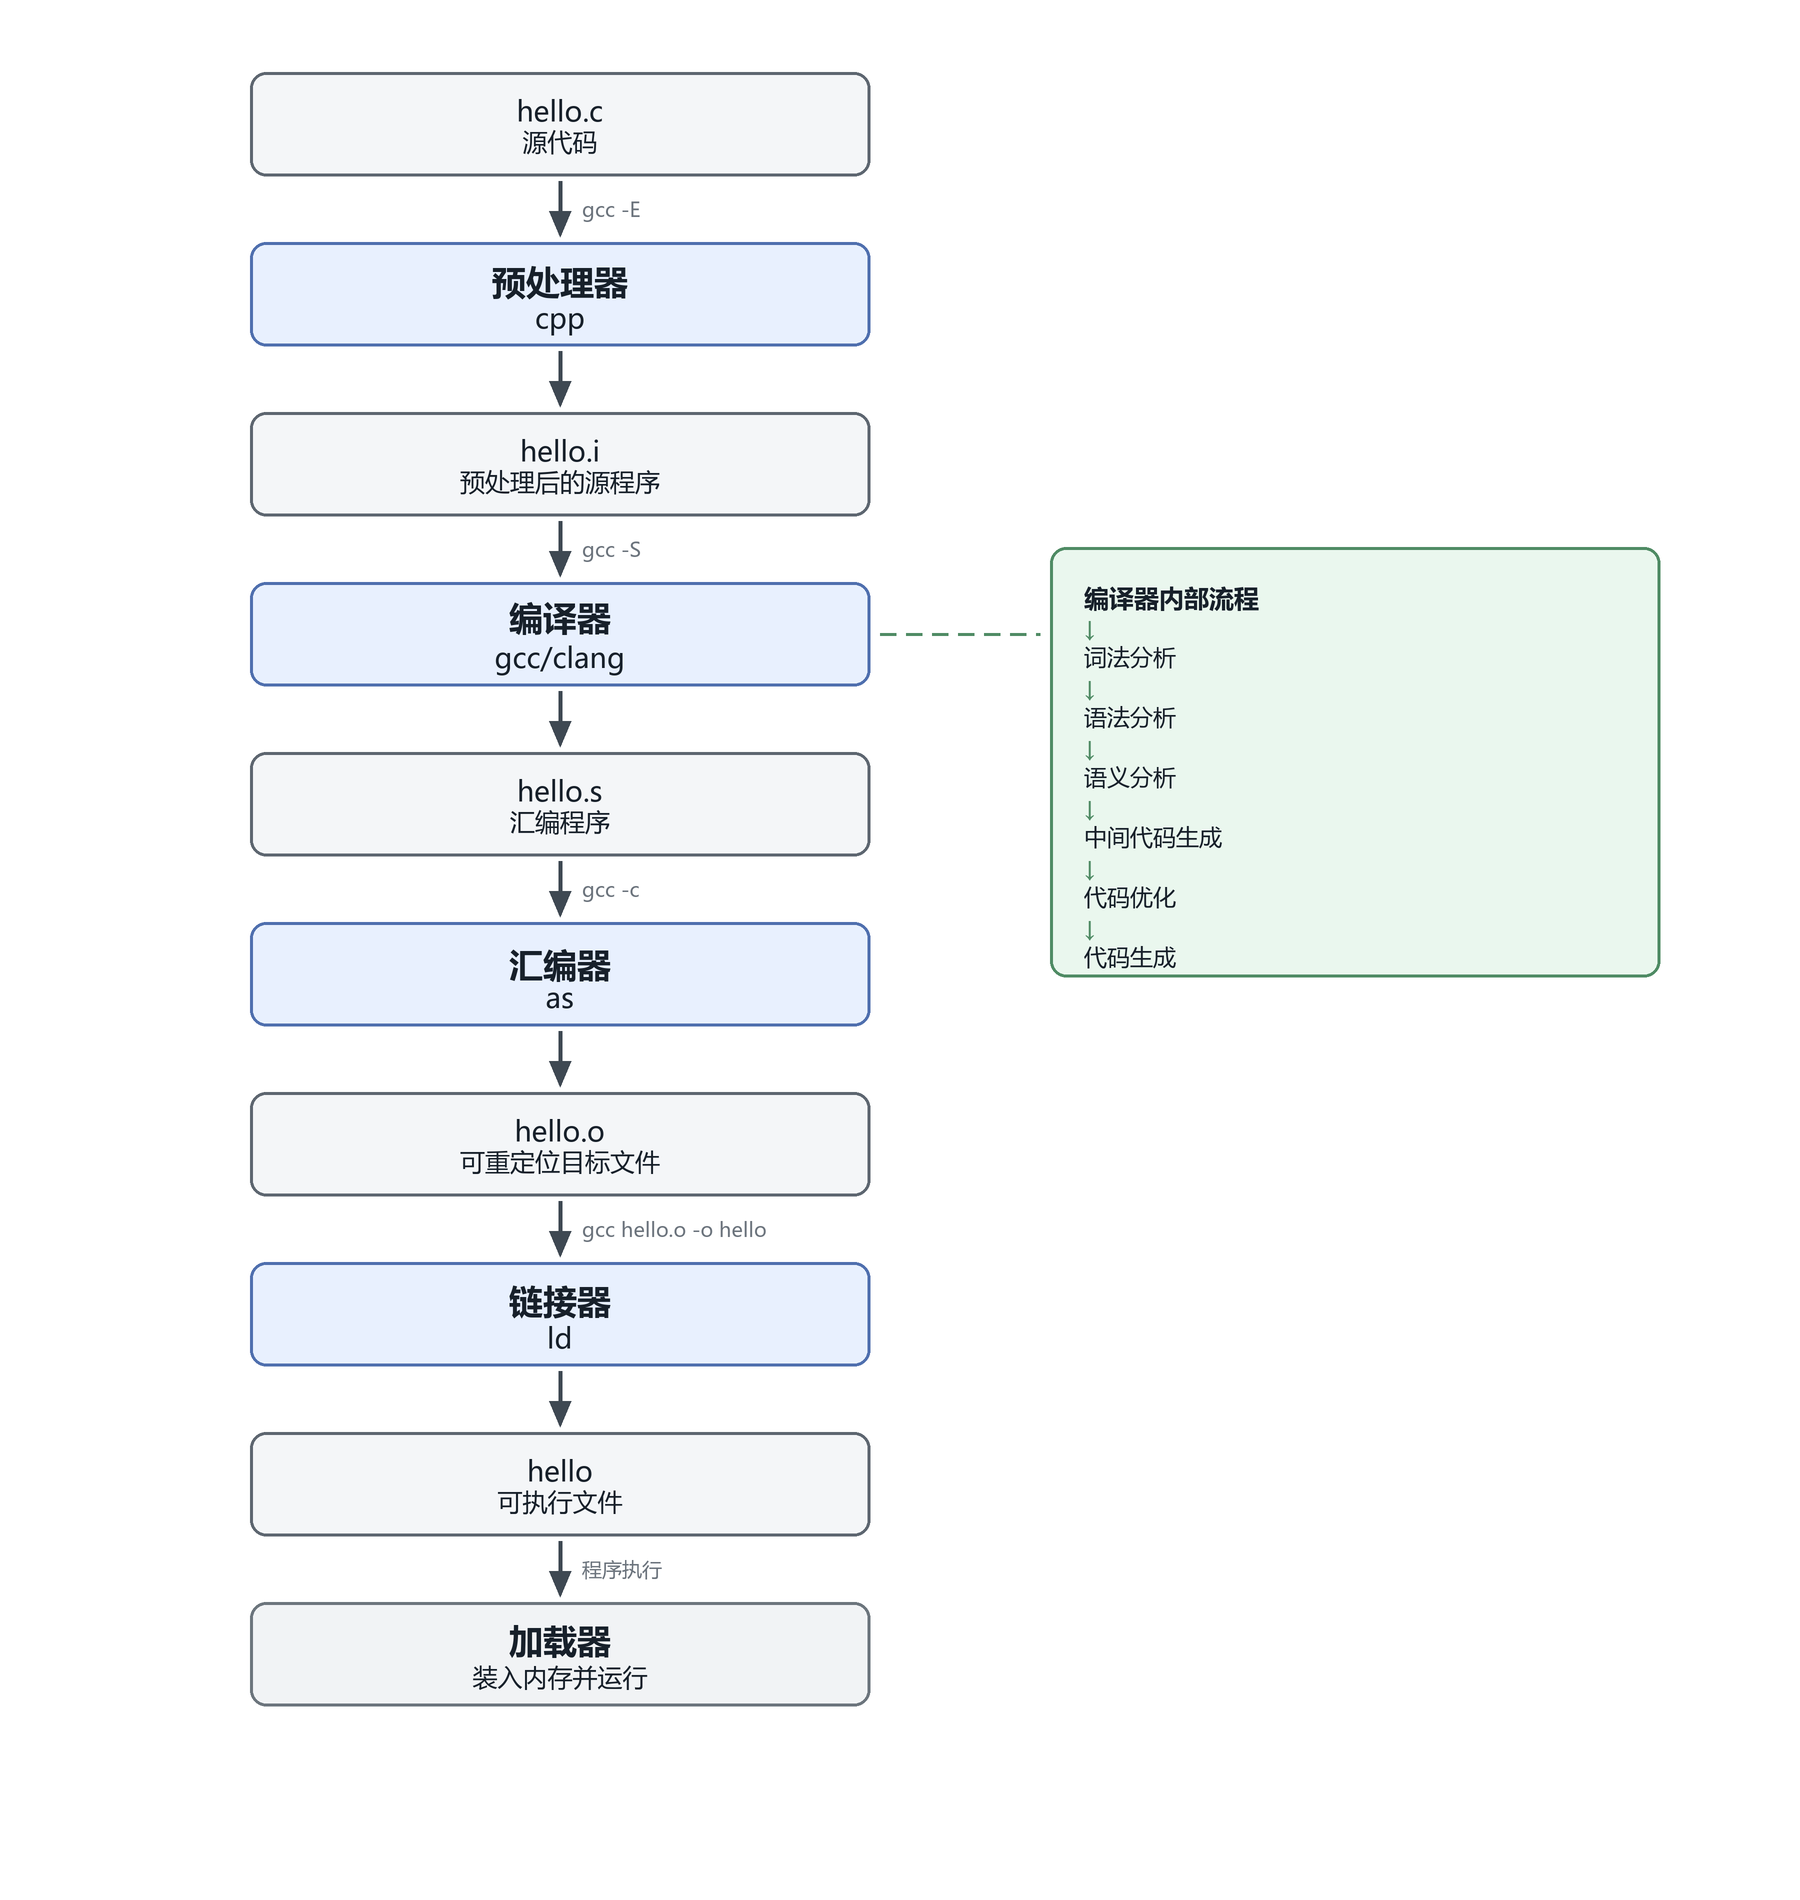
\includegraphics[width=0.5\linewidth]{images/compilation process.png}
        \caption{编译过程}
        \label{fig:编译过程}
\end{figure}    

编写main.c文件来对编译过程进行测试，程序源码如下所示：

\begin{minted}[frame=single, linenos=true]{c}
main()
{
    int a,b,i,t,n;
    a=0;
    b=1;
    i=1;
    cin>>n;
    cout<<a<<endl;
    cout<<b<<endl;
    while(i<n)
    {
        t=b;
        b=a+b;
        cout<<b<<endl;
        a=t;
        i=i+1;
    }
}
\end{minted}
使用\textbf{clang -ccc-print-phases main.c}指令，得到编译的整个流程，如图\ref{fig:main.c编译}所示。
    \begin{figure}[H]
        \centering
        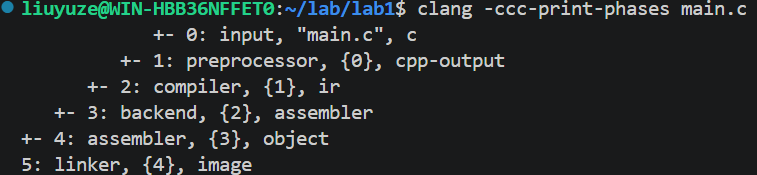
\includegraphics[width=0.8\linewidth]{images/main.c_compilation.png}
        \caption{main.c编译}
        \label{fig:main.c编译}
    \end{figure}
    
\textbf{完全符合我们所学到的编译流程。}

\subsubsection{预处理器}

\textbf{(1)预处理阶段的功能}
\begin{itemize}[leftmargin=*]
  \item \textbf{处理预处理指令}

  处理源代码中以 \verb|#| 开头的指令，例如 \verb|#include|、\verb|#define|、
  \verb|#if| 等。

  \item \textbf{展开头文件和宏定义}

  对于 \verb|#include|，将对应头文件的内容插入源文件；对于 \verb|#define|，
  将宏在代码中出现的位置替换为相应内容。

  \item \textbf{处理条件编译}

  根据 \verb|#if| 等条件编译指令，决定哪些代码参与后续编译、哪些代码被忽略。

  \item \textbf{清理和标记源代码}

  删除源代码中的注释，并添加行号、文件名等标识，以便后续编译器定位和处理代码。

  \item \textbf{生成预处理后的源程序}

  预处理器的输出不是汇编代码或机器代码，而是经过头文件插入、宏展开和条件选择后的源程序。

  \item \textbf{作为编译流程的第一个阶段}

  预处理结果会交给编译器继续进行词法分析、语法分析、语义分析、中间代码生成等工作。
  
\end{itemize}

\textbf{(2)实验验证}

为了验证预处理器的主要功能，本实验在原斐波那契数列程序的基础上进行了修改。首先，
在源文件开头加入 \verb|#include <stdio.h>|，以使用 C 语言中的 \verb|scanf| 和
\verb|printf| 完成输入输出。其次，使用 \verb|#define| 定义宏常量
\verb|FIB_A0|、\verb|FIB_B0|、\verb|FIB_I0| 以及函数宏 \verb|FIB_NEXT(x)|，
并将程序中的相关赋值和循环变量更新替换为这些宏，以便观察宏替换的结果。同时，
在代码中加入单行注释和多行注释，用于验证预处理器对注释的处理；并通过
\verb|#ifdef FIB_DEBUG| 加入调试输出语句，用于验证条件编译功能。

修改后的代码如下所示

\begin{minted}[frame=single, linenos=true]{c}
#include <stdio.h>

// FIB_SINGLE_COMMENT

/* FIB_BLOCK_COMMENT */

#define FIB_A0 0
#define FIB_B0 1
#define FIB_I0 1
#define FIB_NEXT(x) ((x) + 1)

int main()
{
    int a, b, i, t, n;

    a = FIB_A0;
    b = FIB_B0;
    i = FIB_I0;

    scanf("%d", &n);

    printf("%d\n", a);
    printf("%d\n", b);

#ifdef FIB_DEBUG
    printf("debug\n");
#endif

    while (i < n)
    {
        t = b;
        b = a + b;

        printf("%d\n", b);

        a = t;
        i = FIB_NEXT(i);
    }

    return 0;
}
\end{minted}

完成修改后，执行

\begin{verbatim}
gcc main.c -E -o main.i
\end{verbatim}

得到预处理后的文件 \verb|main.i|。通过对比源文件和预处理结果，可以进一步分析
头文件展开、宏替换、注释删除以及条件编译等预处理功能：

\begin{figure}[H]
        \centering
        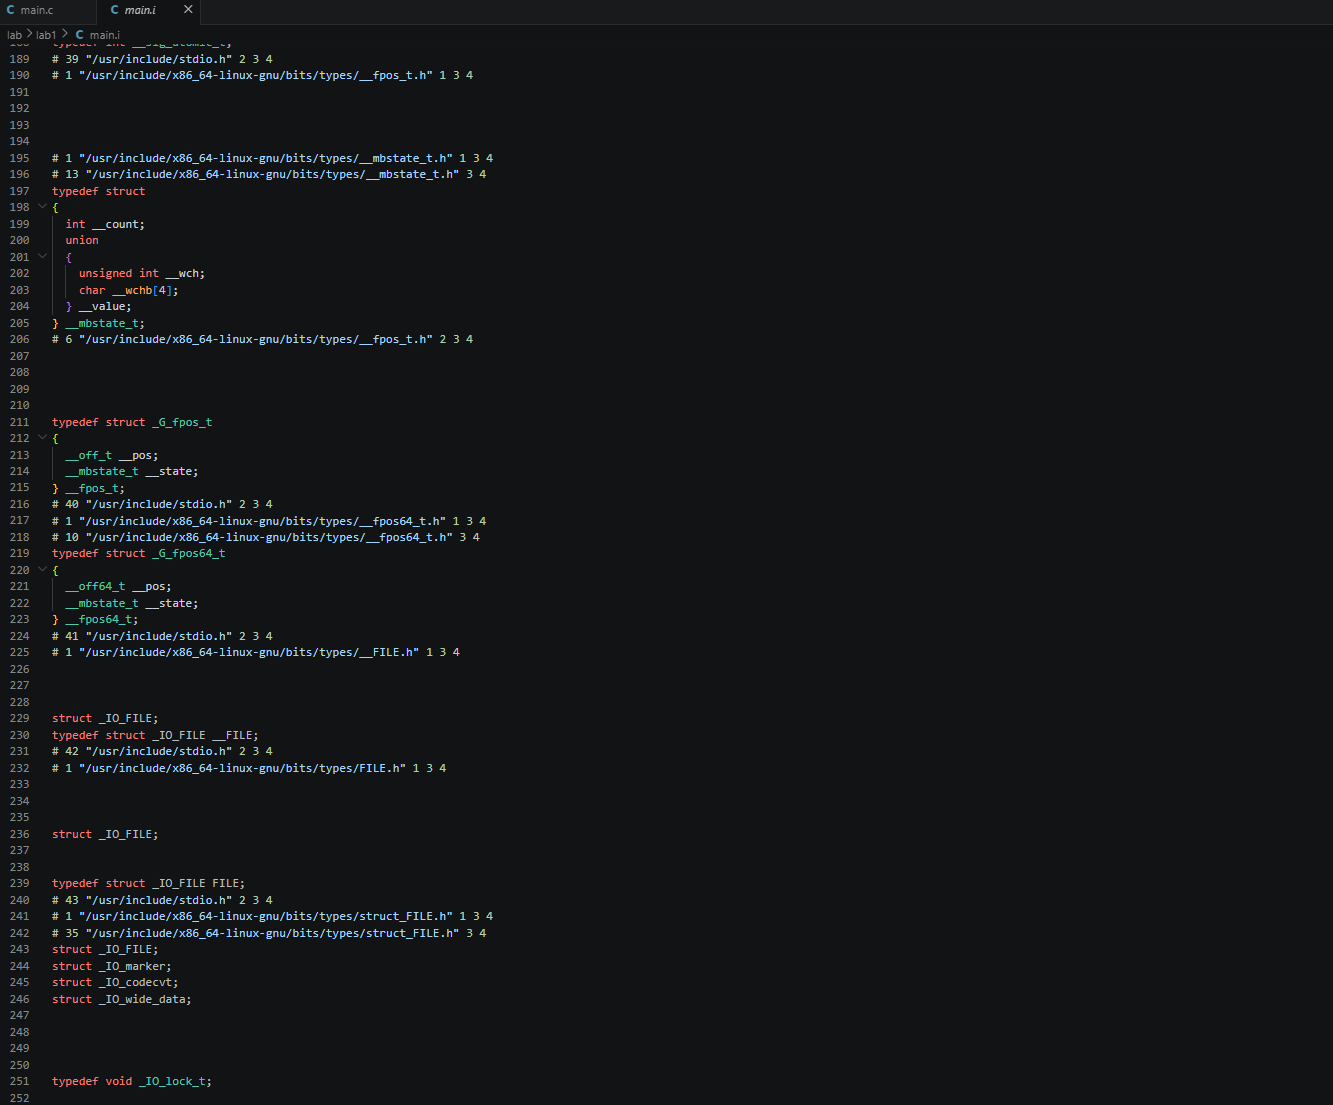
\includegraphics[width=0.8\linewidth]{images/processed_code.png}
        \caption{预处理后的代码}
        \label{fig:预处理后的代码}
\end{figure}





\subsubsection{编译器}


\textbf{(1)词法分析}

词法分析的主要功能是：从左到右扫描预处理后的源程序，将其中的字符序列划分为具有
明确类别的词法单元（Token），例如关键字、标识符、常量、运算符和分隔符，并记录它
们在源程序中的位置，为后续的语法分析提供输入。

本节使用经过预处理的 \verb|main.c|，执行如下命令：

\begin{minted}{bash}
clang -E -Xclang -dump-tokens main.c
\end{minted}

该命令会在预处理的基础上输出词法分析结果。部分结果如图
\ref{fig:lexical-analysis} 所示。

\begin{figure}[H]
    \centering
    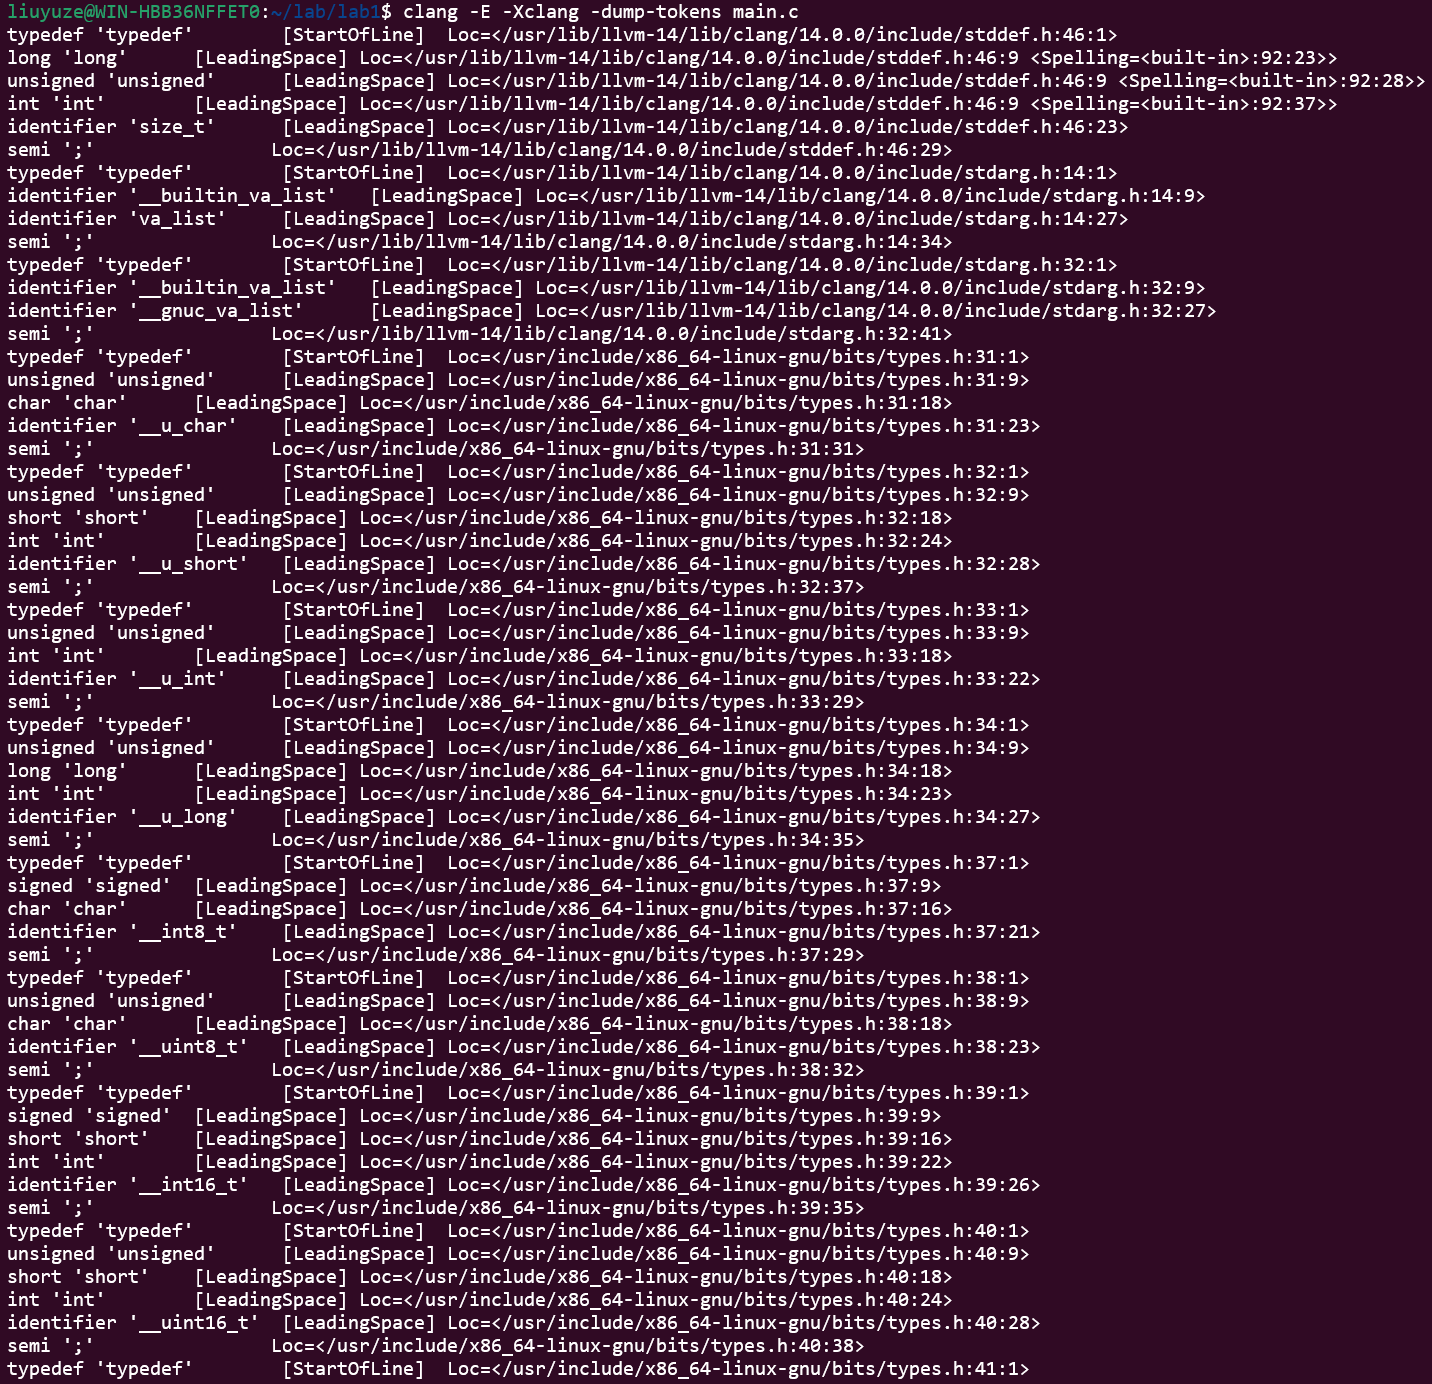
\includegraphics[width=0.8\linewidth]{images/lexer_result.png}
    \caption{词法分析结果}
    \label{fig:lexical-analysis}
\end{figure}

以下截取 \verb|main| 函数附近的典型部分进行分析。

\begin{enumerate}[label=\roman*.]
    \item 主函数与变量声明

\begin{lstlisting}[style=asm]
int 'int'        [StartOfLine]  Loc=<main.c:12:1>
identifier 'main' [LeadingSpace] Loc=<main.c:12:5>
l_paren '('       Loc=<main.c:12:9>
r_paren ')'       Loc=<main.c:12:10>
l_brace '{'       [StartOfLine] Loc=<main.c:13:1>
int 'int'         [StartOfLine] [LeadingSpace] Loc=<main.c:14:5>
identifier 'a'    [LeadingSpace] Loc=<main.c:14:9>
comma ','         Loc=<main.c:14:10>
identifier 'b'    [LeadingSpace] Loc=<main.c:14:12>
comma ','         Loc=<main.c:14:13>
identifier 'i'    [LeadingSpace] Loc=<main.c:14:15>
comma ','         Loc=<main.c:14:16>
identifier 't'    [LeadingSpace] Loc=<main.c:14:18>
comma ','         Loc=<main.c:14:19>
identifier 'n'    [LeadingSpace] Loc=<main.c:14:21>
semi ';'          Loc=<main.c:14:22>
\end{lstlisting}

这里，\verb|int| 被识别为关键字，\verb|main|、\verb|a|、\verb|b|、\verb|i|、
\verb|t| 和 \verb|n| 被识别为标识符；左右括号、左右花括号分别用于表示参数列表和
函数体，逗号表示变量之间的分隔，分号表示一条声明语句的结束。

    \item 赋值、输入输出与运算符

\begin{lstlisting}[style=asm]
identifier 'a'             [StartOfLine] [LeadingSpace] Loc=<main.c:16:5>
equal '='                  [LeadingSpace] Loc=<main.c:16:7>
numeric_constant '0'       [LeadingSpace]
                           Loc=<main.c:16:9 <Spelling=main.c:7:16>>
semi ';'                   Loc=<main.c:16:15>
identifier 'scanf'         [StartOfLine] [LeadingSpace] Loc=<main.c:20:5>
l_paren '('                Loc=<main.c:20:10>
string_literal '"%d"'      Loc=<main.c:20:11>
comma ','                  Loc=<main.c:20:15>
amp '&'                    [LeadingSpace] Loc=<main.c:20:17>
identifier 'n'             Loc=<main.c:20:18>
r_paren ')'                Loc=<main.c:20:19>
semi ';'                   Loc=<main.c:20:20>
identifier 'printf'        [StartOfLine] [LeadingSpace] Loc=<main.c:22:5>
l_paren '('                Loc=<main.c:22:11>
string_literal '"%d\n"'    Loc=<main.c:22:12>
comma ','                  Loc=<main.c:22:18>
identifier 'a'             [LeadingSpace] Loc=<main.c:22:20>
r_paren ')'                Loc=<main.c:22:21>
semi ';'                   Loc=<main.c:22:22>
\end{lstlisting}

赋值号被识别为 \verb|equal|，加号被识别为 \verb|plus|；取地址符号被识别为
\verb|amp|。\verb|scanf| 和 \verb|printf| 是标识符，而 \verb|"%d"| 与
\verb|"%d\n"| 是完整的字符串常量。后者中的 \verb|\n| 属于字符串字面量的一部分，
不会被拆分成独立的词法单元。

宏常量 \verb|FIB_A0| 已在此前的预处理阶段被替换为数值常量 \verb|0|。输出中的
\verb|Spelling=main.c:7:16| 说明了该数值来源于 \verb|#define FIB_A0 0| 所在的
位置，因此词法分析器接收到的内容已经是宏展开后的代码。

    \item 循环、宏函数展开与程序结束

\begin{lstlisting}[style=asm]
while 'while'             [StartOfLine] [LeadingSpace] Loc=<main.c:29:5>
l_paren '('               [LeadingSpace] Loc=<main.c:29:11>
identifier 'i'            Loc=<main.c:29:12>
less '<'                  [LeadingSpace] Loc=<main.c:29:14>
identifier 'n'            [LeadingSpace] Loc=<main.c:29:16>
r_paren ')'               Loc=<main.c:29:17>
l_brace '{'               [StartOfLine] [LeadingSpace] Loc=<main.c:30:5>
identifier 't'            [StartOfLine] [LeadingSpace] Loc=<main.c:31:9>
equal '='                 [LeadingSpace] Loc=<main.c:31:11>
identifier 'b'            [LeadingSpace] Loc=<main.c:31:13>
semi ';'                  Loc=<main.c:31:14>
identifier 'b'            [StartOfLine] [LeadingSpace] Loc=<main.c:32:9>
equal '='                 [LeadingSpace] Loc=<main.c:32:11>
identifier 'a'            [LeadingSpace] Loc=<main.c:32:13>
plus '+'                  [LeadingSpace] Loc=<main.c:32:15>
identifier 'b'            [LeadingSpace] Loc=<main.c:32:17>
semi ';'                  Loc=<main.c:32:18>
identifier 'i'            [StartOfLine] [LeadingSpace] Loc=<main.c:37:9>
equal '='                 [LeadingSpace] Loc=<main.c:37:11>
l_paren '('               [LeadingSpace]
                          Loc=<main.c:37:13 <Spelling=main.c:10:21>>
l_paren '('               Loc=<main.c:37:13 <Spelling=main.c:10:22>>
identifier 'i'            Loc=<main.c:37:13 <Spelling=main.c:37:22>>
r_paren ')'               Loc=<main.c:37:13 <Spelling=main.c:10:24>>
plus '+'                  [LeadingSpace]
                          Loc=<main.c:37:13 <Spelling=main.c:10:26>>
numeric_constant '1'      [LeadingSpace]
                          Loc=<main.c:37:13 <Spelling=main.c:10:28>>
r_paren ')'               Loc=<main.c:37:13 <Spelling=main.c:10:29>>
semi ';'                  Loc=<main.c:37:24>
return 'return'           [StartOfLine] [LeadingSpace] Loc=<main.c:40:5>
numeric_constant '0'      [LeadingSpace] Loc=<main.c:40:12>
semi ';'                  Loc=<main.c:40:13>
r_brace '}'               [StartOfLine] Loc=<main.c:41:1>
eof ''                    Loc=<main.c:41:2>
\end{lstlisting}

\verb|while| 和 \verb|return| 被识别为关键字，小于号被识别为 \verb|less|，
加号被识别为 \verb|plus|。\verb|FIB_NEXT(i)| 在预处理阶段被展开为
\verb|((i) + 1)|，因此词法分析结果中出现的是括号、标识符 \verb|i|、加号和数值
常量 \verb|1|，而不是单个名为 \verb|FIB_NEXT| 的词法单元。

输出中没有出现单行注释、多行注释以及 \verb|#ifdef FIB_DEBUG| 控制的调试输出。
这是因为本节执行的是预处理后的词法分析：注释已经在预处理阶段被删除，而未定义
\verb|FIB_DEBUG| 时，调试输出语句也不会进入预处理结果。最后的 \verb|eof| 表示
词法分析器已经扫描到输入文件的末尾。
\end{enumerate}

综上，源程序被成功分解为具有明确类别和位置信息的词法单元；宏定义和条件编译已在
词法分析之前处理，函数宏 \verb|FIB_NEXT(i)| 也被展开为普通的括号、运算符和常量
序列。由此验证了词法分析将字符流转换为 Token 序列的功能。

\textbf{(2)语法分析}

语法分析的主要功能是：以前一步词法分析产生的 Token 序列作为输入，根据 C 语言的语法规则识别程序的层次结构，并构造抽象语法树（Abstract Syntax Tree，AST）。
使用如下命令生成 AST：

\begin{minted}{bash}
clang -E -Xclang -ast-dump main.c
\end{minted}

终端部分结果如图 \ref{fig:syntax-analysis} 所示。

\begin{figure}[H]
        \centering
        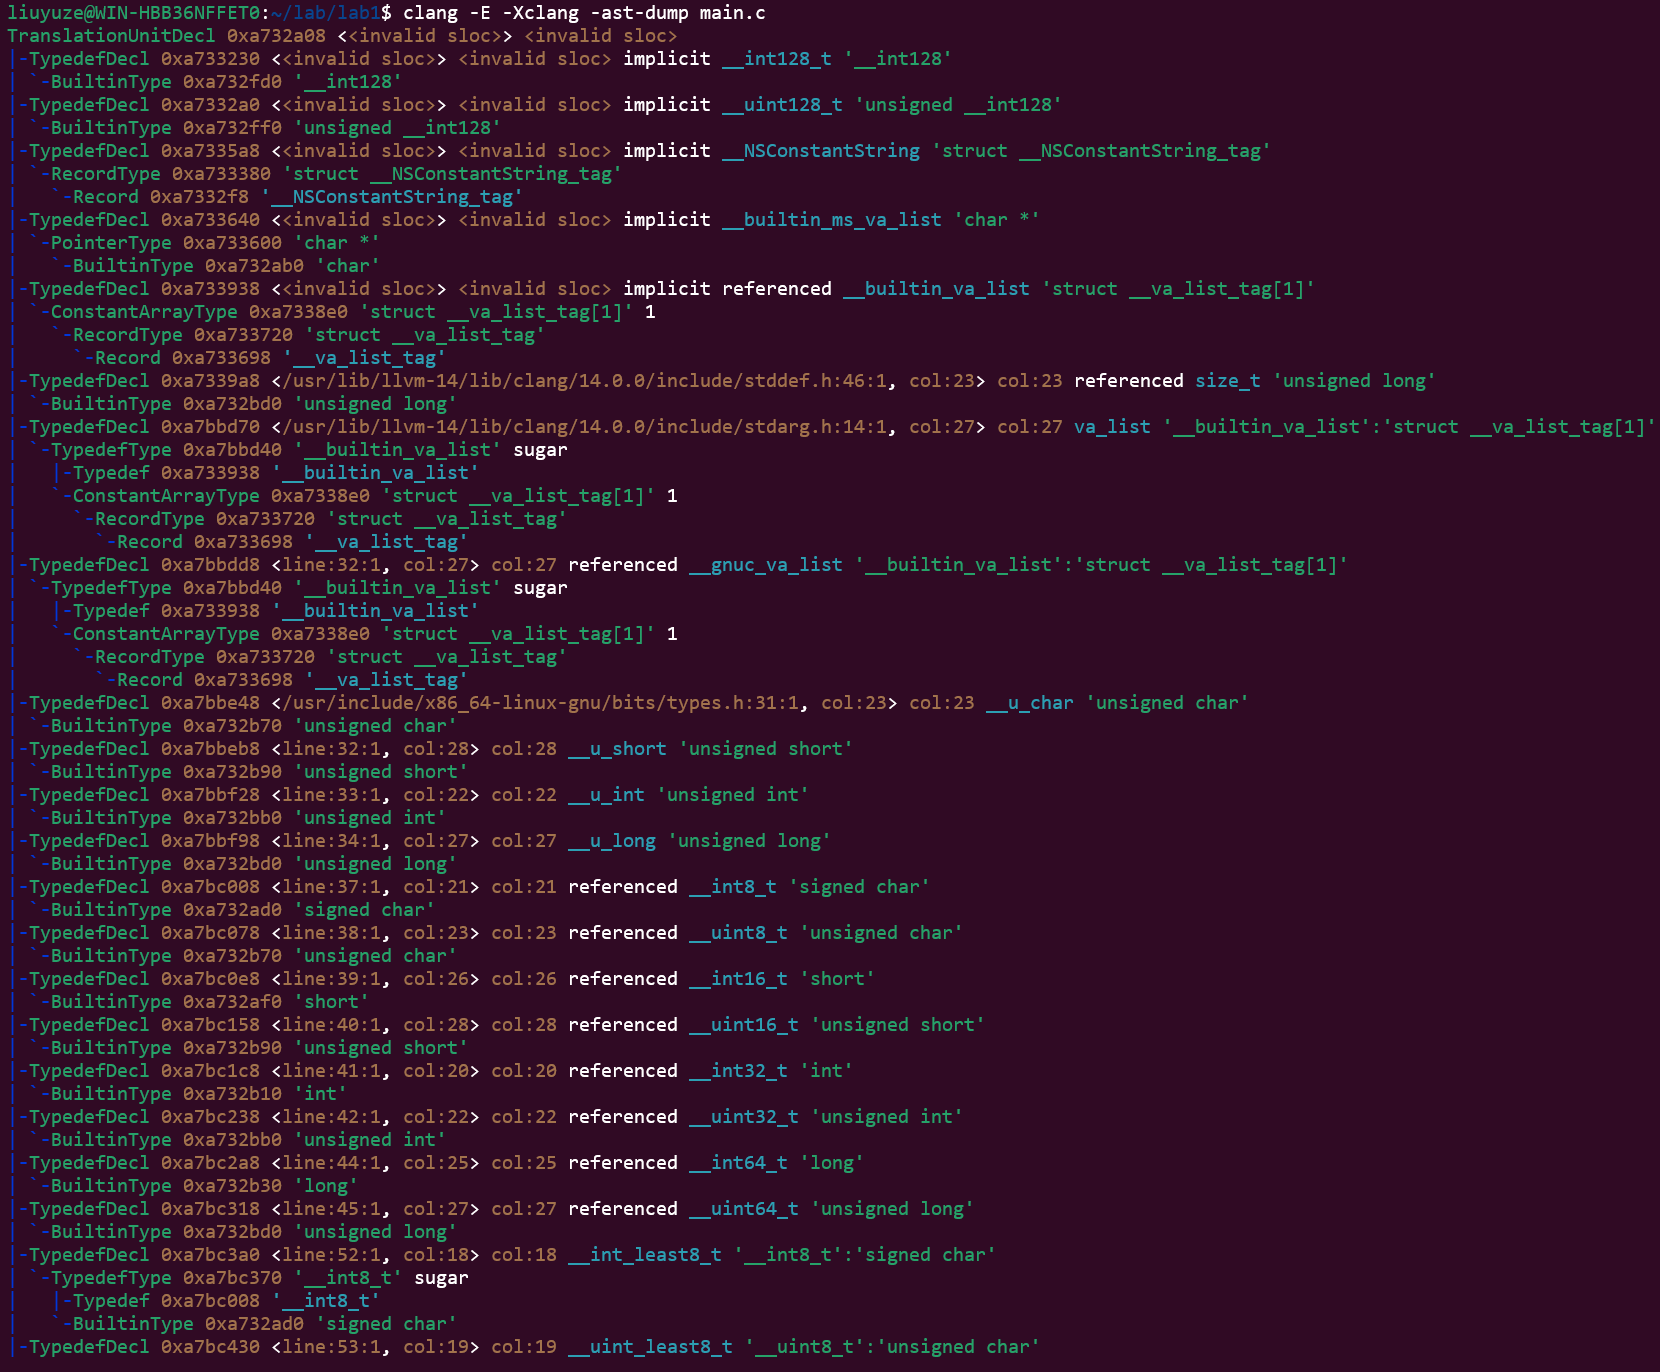
\includegraphics[width=0.8\linewidth]{images/syntax_analysis.png}
        \caption{语法分析结果}
        \label{fig:syntax-analysis}
\end{figure}

\begin{enumerate}[label=\roman*.]
    \item 主函数、函数体与变量声明

\begin{lstlisting}[style=asm]
`-FunctionDecl 0x1dcfe760 <main.c:12:1, line:41:1> line:12:5 main 'int ()'
  `-CompoundStmt 0x1dcff998 <line:13:1, line:41:1>
    |-DeclStmt 0x1dcfeab0 <line:14:5, col:22>
    | |-VarDecl 0x1dcfe818 <col:5, col:9> col:9 used a 'int'
    | |-VarDecl 0x1dcfe898 <col:5, col:12> col:12 used b 'int'
    | |-VarDecl 0x1dcfe918 <col:5, col:15> col:15 used i 'int'
    | |-VarDecl 0x1dcfe998 <col:5, col:18> col:18 used t 'int'
    | `-VarDecl 0x1dcfea18 <col:5, col:21> col:21 used n 'int'
\end{lstlisting}

最上层的 \verb|FunctionDecl| 表示函数声明，节点名称 \verb|main| 和类型
\verb|'int ()'| 说明程序中定义了一个返回值为 \verb|int|、不接收参数的
\verb|main| 函数。它下面的 \verb|CompoundStmt| 是复合语句节点，对应
\verb|main| 函数的一对花括号，表示函数的整个函数体。

在函数体中，\verb|DeclStmt| 表示一条变量声明语句，其下的五个
\verb|VarDecl| 分别表示变量 \verb|a|、\verb|b|、\verb|i|、\verb|t| 和
\verb|n|。每个节点后方的 \verb|'int'| 表示变量的类型为整型；
\verb|used| 表示该变量在后续代码中确实被使用，而各个位置字段则用于记录变量
声明在源程序中的位置。

    \item 赋值、输入输出与函数调用

\begin{lstlisting}[style=asm]
|-BinaryOperator 0x1dcfeb08 <line:16:5, line:7:16> 'int' '='
| |-DeclRefExpr 0x1dcfeac8 <line:16:5> 'int' lvalue Var 0x1dcfe818 'a' 'int'
| `-IntegerLiteral 0x1dcfeae8 <line:7:16> 'int' 0
|-CallExpr 0x1dcff250 <line:20:5, col:19> 'int'
| |-ImplicitCastExpr 0x1dcff238 <col:5>
| | `-DeclRefExpr 0x1dcfebe8 <col:5> Function 0x1dcf3bc0 'scanf'
| |-ImplicitCastExpr 0x1dcff280 <col:11> 'char *' <ArrayToPointerDecay>
| | `-StringLiteral 0x1dcfec48 <col:11> 'char[3]' lvalue "%d"
| `-UnaryOperator 0x1dcff1a8 <col:17, col:18> 'int *' prefix '&'
|   `-DeclRefExpr 0x1dcfec68 <col:18> 'int' lvalue Var 0x1dcfea18 'n' 'int'
|-CallExpr 0x1dcff340 <line:22:5, col:21> 'int'
| |-ImplicitCastExpr 0x1dcff328 <col:5>
| | `-DeclRefExpr 0x1dcff2b0 <col:5> Function 0x1dce3578 'printf'
| |-ImplicitCastExpr 0x1dcff370 <col:12> 'char *' <ArrayToPointerDecay>
| | `-StringLiteral 0x1dcff2d0 <col:12> 'char[4]' lvalue "%d\n"
| `-ImplicitCastExpr 0x1dcff3a0 <col:20> 'int' <LValueToRValue>
|   `-DeclRefExpr 0x1dcff2f0 <col:20> 'int' lvalue Var 0x1dcfe818 'a' 'int'
\end{lstlisting}

\verb|BinaryOperator| 表示二元运算。在 \verb|a = 0| 的节点中，赋值号左侧的
\verb|DeclRefExpr| 表示对变量 \verb|a| 的引用，右侧的
\verb|IntegerLiteral| 表示整数常量 \verb|0|。需要注意的是，该常量的位置来自
\verb|main.c| 第 7 行的宏定义，说明 \verb|FIB_A0| 已经在预处理阶段被替换为
\verb|0|，语法分析直接处理的是宏展开后的结果。

\verb|CallExpr| 表示函数调用。\verb|scanf| 调用中包含字符串字面量
\verb|"%d"|、取地址运算符 \verb|&| 以及变量 \verb|n| 的引用，分别对应源程序
中的格式字符串和 \verb|&n|。同样，两个 \verb|printf| 调用中包含字符串字面量
\verb|"%d\n"|，并通过 \verb|DeclRefExpr| 引用变量 \verb|a| 或 \verb|b|，从
而确定了输出语句的语法结构。

\verb|ImplicitCastExpr| 并没有直接写在源程序中，而是编译器根据类型规则自动
加入的隐式转换节点。例如，函数名需要转换为函数指针，数组形式的字符串需要转换
为字符指针，变量从存储位置读取数值时则会产生 \verb|LValueToRValue| 转换。

    \item while 循环、循环体与宏函数展开

\begin{lstlisting}[style=asm]
|-WhileStmt 0x1dcff948 <line:29:5, line:38:5>
| |-BinaryOperator 0x1dcff530 <line:29:12, col:16> 'int' '<'
| | |-ImplicitCastExpr 0x1dcff500 <col:12> 'int' <LValueToRValue>
| | | `-DeclRefExpr 0x1dcff4c0 <col:12> 'int' lvalue Var 0x1dcfe918 'i'
| | `-ImplicitCastExpr 0x1dcff518 <col:16> 'int' <LValueToRValue>
| |   `-DeclRefExpr 0x1dcff4e0 <col:16> 'int' lvalue Var 0x1dcfea18 'n'
| `-CompoundStmt 0x1dcff910 <line:30:5, line:38:5>
|   |-BinaryOperator 0x1dcff5a8 <line:31:9, col:13> 'int' '='
|   | |-DeclRefExpr 0x1dcff550 <col:9> 'int' lvalue Var 0x1dcfe998 't'
|   | `-DeclRefExpr 0x1dcff570 <col:13> 'int' lvalue Var 0x1dcfe898 'b'
|   |-BinaryOperator 0x1dcff678 <line:32:9, col:17> 'int' '='
|   | |-DeclRefExpr 0x1dcff5c8 <col:9> 'int' lvalue Var 0x1dcfe898 'b'
|   | `-BinaryOperator 0x1dcff658 <col:13, col:17> 'int' '+'
|   |   |-DeclRefExpr 0x1dcff5e8 <col:13> 'int' lvalue Var 0x1dcfe818 'a'
|   |   `-DeclRefExpr 0x1dcff608 <col:17> 'int' lvalue Var 0x1dcfe898 'b'
|   `-BinaryOperator 0x1dcff8f0 <line:37:9, line:10:29> 'int' '='
|     |-DeclRefExpr 0x1dcff818 <line:37:9> 'int' lvalue Var 0x1dcfe918 'i'
|     `-ParenExpr 0x1dcff8d0 <line:10:21, col:29> 'int'
|       `-BinaryOperator 0x1dcff8b0 <col:22, col:28> 'int' '+'
|         |-ParenExpr 0x1dcff858 <col:22, col:24> 'int' lvalue
|         | `-DeclRefExpr 0x1dcff838 <line:37:22> 'int' lvalue Var 'i'
|         `-IntegerLiteral 0x1dcff878 <line:10:28> 'int' 1
`-ReturnStmt 0x1dcff988 <line:40:5, col:12>
  `-IntegerLiteral 0x1dcff968 <col:12> 'int' 0
\end{lstlisting}

\verb|WhileStmt| 表示循环语句。它下面有两个主要子树：第一个是以
\verb|<| 为运算符的 \verb|BinaryOperator|，对应循环条件 \verb|i < n|；第二个是 \verb|CompoundStmt|，对应花括号包围的循环体。循环体中的循环变量更新、临时变量赋值和加法运算也都被构造成层次分明的 \verb|BinaryOperator| 节点。

在 \verb|i = FIB_NEXT(i)| 对应的节点中，没有出现名为 \verb|FIB_NEXT| 的函数
调用。预处理阶段已将 \verb|FIB_NEXT(i)| 展开为 \verb|((i) + 1)|，因此 AST 中
表现为外侧的 \verb|ParenExpr|、中间的加法 \verb|BinaryOperator|、变量
\verb|i| 所对应的 \verb|DeclRefExpr| 以及整数常量 \verb|1|。这一结构直接验证了
函数宏展开确实发生在语法分析之前。

最后，\verb|ReturnStmt| 表示返回语句，其下的 \verb|IntegerLiteral 0| 对应
\verb|return 0|。AST 中也没有出现 \verb|#ifdef FIB_DEBUG| 控制的调试输出，因为
本次编译没有定义 \verb|FIB_DEBUG|，条件编译块在预处理阶段已被移除。
\end{enumerate}

综上，Clang 将预处理后的 Token 序列成功组织成了具有层次关系的抽象语法树。
函数定义、变量声明、赋值、函数调用、选择结构和循环结构都能在 AST 中找到对应的
节点，说明语法分析器已经正确识别了源程序的语法结构，并为后续语义分析提供了
基础。

\textbf{语法错误检查验证}

为了进一步验证语法分析器检查语法错误的功能，可以另外建立一个
\verb|test_syntax.c|：

\begin{minted}[frame=single, linenos=true]{c}
int main()
{
    int a
    a = 1 + ;
    return 0
}
\end{minted}

执行：

\begin{minted}{bash}
clang -E -Xclang -ast-dump test_syntax.c
\end{minted}

报错结果如图 \ref{fig:syntax-error} 所示。

\begin{figure}[H]
    \centering
    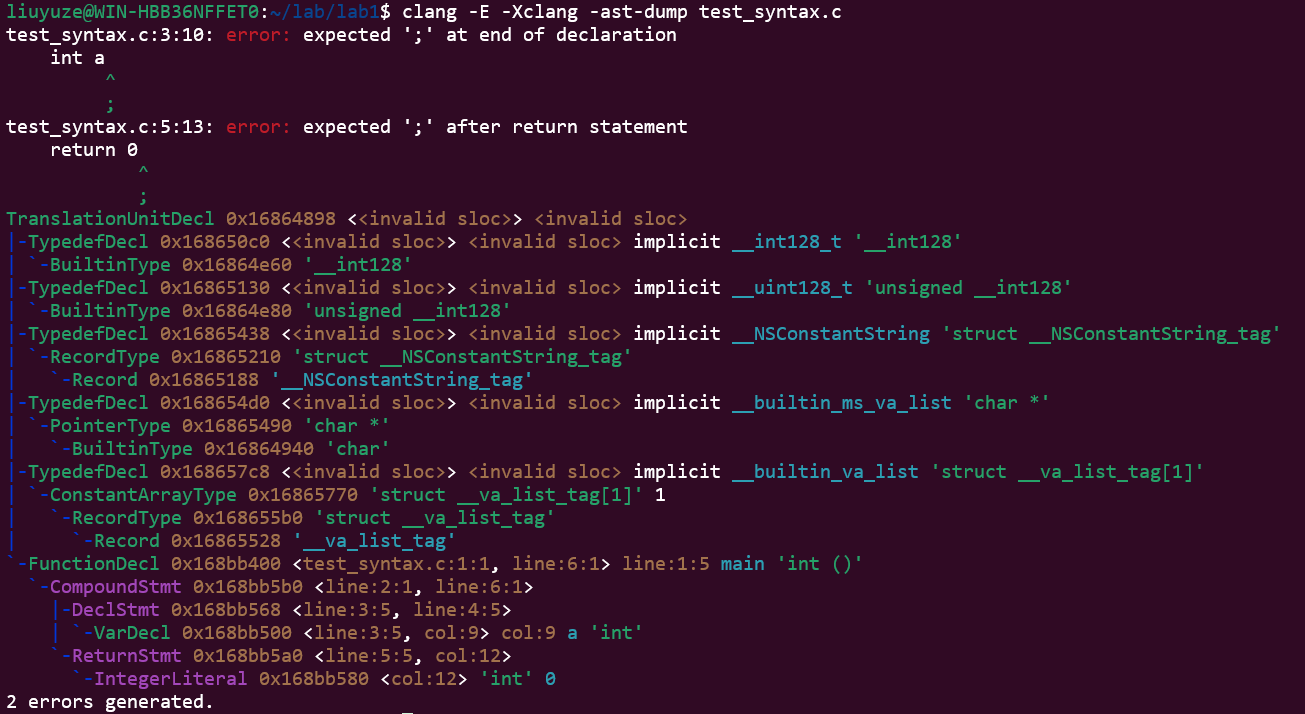
\includegraphics[width=0.8\textwidth]{images/syntax-error.png}
    \caption{语法错误检查结果}
    \label{fig:syntax-error}
\end{figure}

可以观察到，编译器能够指出变量声明后缺少分号、加法表达式缺少右操作数以及
\verb|return| 语句后缺少分号等语法问题。由此说明，语法分析不仅能构造 AST，还能够发现不符合 C 语言语法规则的代码。

\textbf{(3)语义分析}

语义分析的主要功能如下：

\begin{itemize}
    \item \textbf{名称解析：}将变量名、函数名等标识符与抽象语法树中对应的
    声明建立联系，明确每个标识符引用的是哪一个变量或函数。

    \item \textbf{符号表构建与查询：}记录程序中变量和函数的名称、类型、作用域
    等信息，并在使用标识符时通过符号表查找其声明。

    \item \textbf{类型检查：}检查赋值、算术运算、关系运算和函数调用中的类型
    是否兼容，例如赋值号两侧应具有相容的类型，函数实参应与形参匹配。

    \item \textbf{作用域检查：}判断标识符在当前作用域内是否可见，确保局部变量
    只能在其作用域中使用，避免访问未声明的名称。

    \item \textbf{隐式类型转换：}根据 C 语言的类型规则自动插入必要的转换，例如
    函数名转换为函数指针、数组转换为指针以及左值转换为右值。

    \item \textbf{控制流与数据流分析：}分析程序的执行路径和数据传递过程，用于
    发现未初始化变量、不可达代码等问题，并为后续代码优化提供依据。

    \item \textbf{错误检测与报告：}在发现类型不匹配、符号未声明或作用域错误时，
    给出错误所在位置和原因，阻止不满足语义规则的程序继续生成目标代码。
\end{itemize}

使用如下命令对 \verb|main.c| 进行语义检查：

\begin{minted}{bash}
clang -fsyntax-only -Wall -Wextra main.c
\end{minted}

如果终端没有输出错误信息，说明程序中的变量、函数、类型和表达式均通过检查。
检查结果如图 \ref{fig:semantic-analysis} 所示。

\begin{figure}[H]
    \centering
    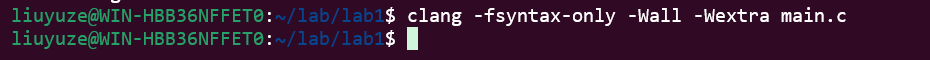
\includegraphics[width=0.8\linewidth]{images/semantic_analysis.png}
    \caption{语义检查成功结果}
    \label{fig:semantic-analysis}
\end{figure}

\textbf{语义错误检查验证}

创建\verb|test_semantic.c| 如下：

\begin{minted}[frame=single, linenos=true]{c}
struct A { int x; };
struct B { int y; };

int f(int x)
{
    return x;
}

void g(struct A value)
{
    (void)value;
}

int conflict(void)
{
    return 0;
}

int conflict(void)
{
    return 1;
}

int main(void)
{
    int a;
    struct B b;

    b = a;
    f();
    g(a);
    unknown = 1;

    int duplicate = 0;
    int duplicate = 1;

    break;
    return 0;
}
\end{minted}

执行：

\begin{minted}{bash}
clang -fsyntax-only test_semantic.c
\end{minted}

检查结果如图 \ref{fig:semantic-error} 所示。


\begin{figure}[H]
    \centering
    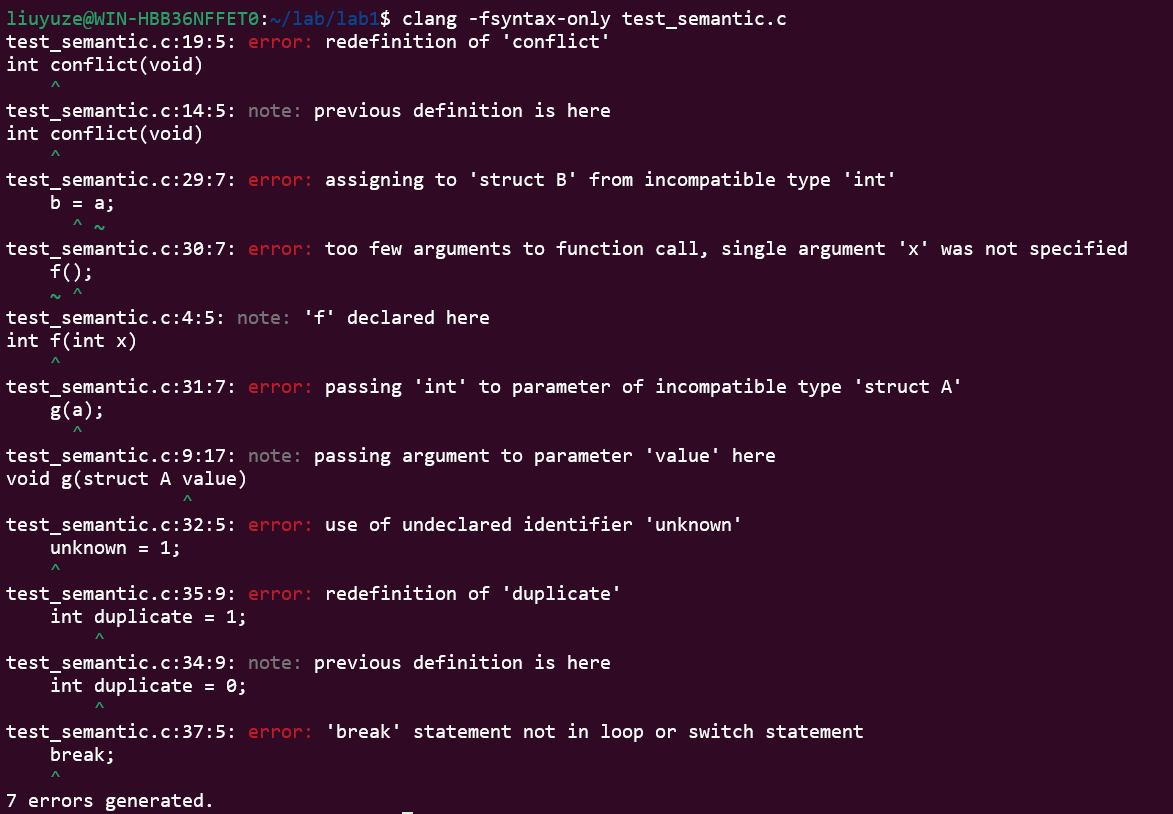
\includegraphics[width=0.8\textwidth]{images/semantic-error.png.png}
    \caption{语义错误检查结果}
    \label{fig:semantic-error}
\end{figure}

综上，Clang 在语法分析生成的 AST 基础上完成了变量与函数的名称解析、表达式类型检查以及函数指针、数组指针和左值到右值等隐式转换。对于不符合语义规则的程序，编译器能够通过符号表和控制流检查发现未声明标识符、类型不兼容、函数调用错误以及符号重复定义等问题，为后续中间代码生成提供正确的语义信息。

\textbf{(4)中间代码生成}

中间代码生成的主要功能是：在语义分析确认源程序合法之后，将抽象语法树转换为
一种与具体目标机器关系较小的中间表示（Intermediate Representation，IR）。
中间表示既要保留源程序中的运算、控制流和数据流信息，又要便于后续进行代码优化
和目标代码生成。本实验所使用的 Clang/LLVM 编译器将 C 源程序转换为 LLVM IR，
其文本形式保存在 \verb|main.ll| 文件中。

中间代码生成的主要功能可以分点说明如下：

\begin{itemize}
    \item \textbf{降低语法树层次：}将具有嵌套结构的表达式和语句转换为一条条
    顺序明确的指令，使程序结构更接近机器能够处理的形式。

    \item \textbf{生成中间表示：}把赋值、算术运算、函数调用和返回等操作转换为
    LLVM IR 指令，例如 \verb|store|、\verb|load|、\verb|add|、\verb|call| 和
    \verb|ret|。

    \item \textbf{构造控制流图：}把条件判断和循环转换为基本块以及基本块之间的
    跳转关系，使用 \verb|br|、\verb|icmp| 等指令表示程序执行路径。

    \item \textbf{保存程序数据信息：}为局部变量分配栈空间，生成相应的
    \verb|alloca|、\verb|load| 和 \verb|store| 指令，并通过虚拟寄存器暂时保存
    中间计算结果。

    \item \textbf{为后续阶段提供输入：}生成的 LLVM IR 与目标机器暂时解耦，既可
    用于代码优化，也可继续生成 x86、ARM 等不同平台的目标代码。
\end{itemize}

本次实验使用如下命令生成 LLVM IR：

\begin{minted}{bash}
clang -S -emit-llvm main.c -o main.ll
\end{minted}

其中，\verb|-S| 表示输出文本形式的代码，\verb|-emit-llvm| 表示生成 LLVM IR，
\verb|-o main.ll| 表示将结果保存到 \verb|main.ll| 文件。命令执行结果如图
\ref{fig:intermediate-code-generation} 所示。

\begin{figure}[H]
    \centering
    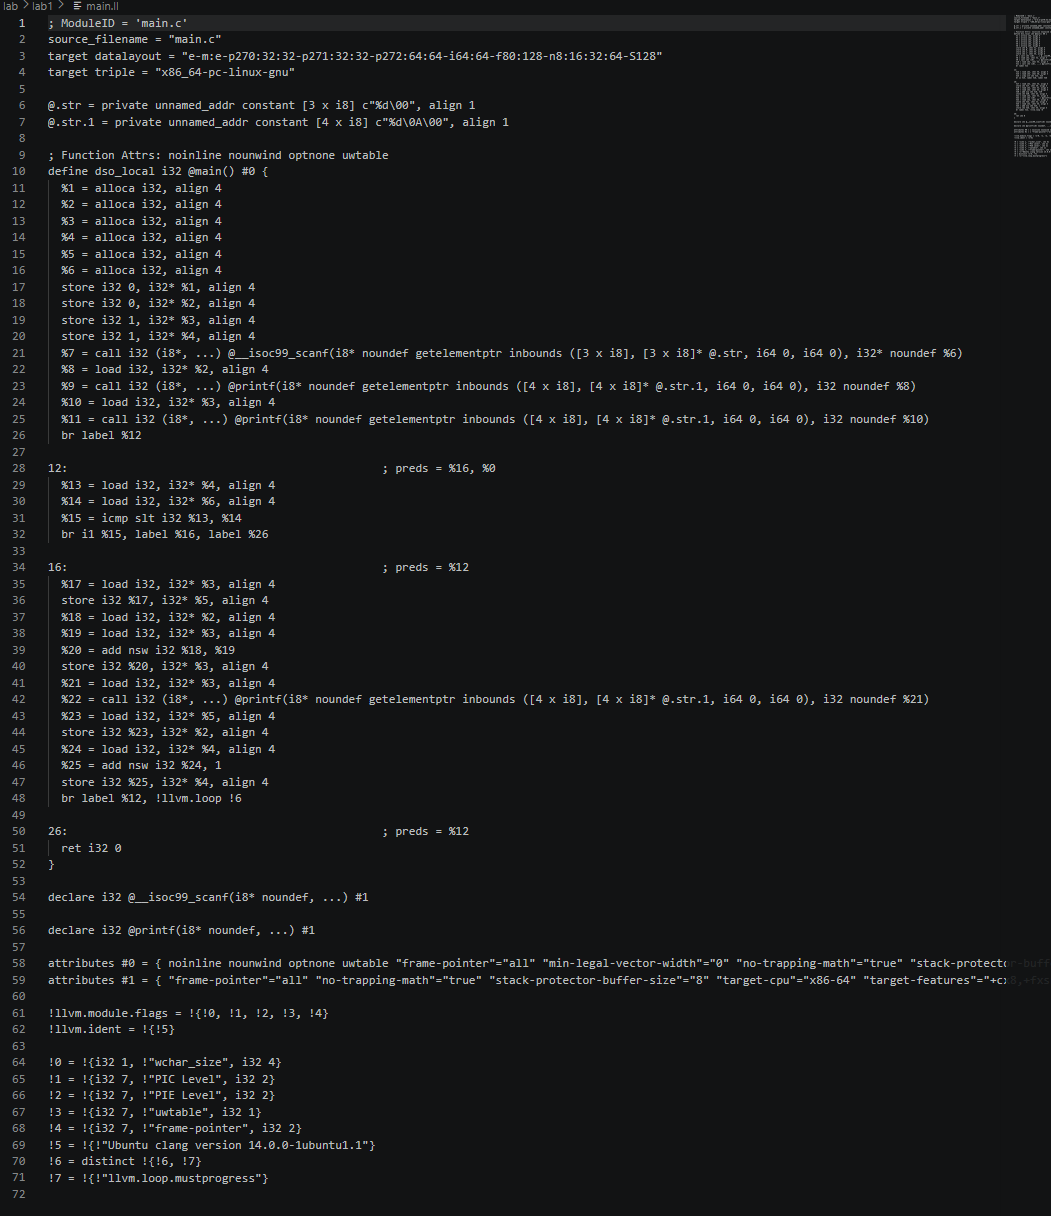
\includegraphics[width=0.6\textwidth]{images/intermediate-code-generation.png}
    \caption{生成main.ll中间代码}
    \label{fig:intermediate-code-generation}
\end{figure}

下面只选取具有代表性的部分进行分析：

\begin{enumerate}[label=\roman*.]
    \item 模块信息与全局字符串

\begin{lstlisting}[style=asm]
; ModuleID = '/home/liuyuze/lab/lab1/main.c'
source_filename = "/home/liuyuze/lab/lab1/main.c"
target datalayout = "e-m:e-p270:32:32-p271:32:32-p272:64:64-i64:64-f80:128-n8:16:32:64-S128"
target triple = "x86_64-pc-linux-gnu"

@.str = private unnamed_addr constant [3 x i8] c"%d\00", align 1
@.str.1 = private unnamed_addr constant [4 x i8] c"%d\0A\00", align 1
\end{lstlisting}

文件开头给出了当前模块的编号、源文件名、目标数据布局和目标三元组。目标三元组
\verb|x86_64-pc-linux-gnu| 说明本次生成的是面向 64 位 x86 Linux 平台的 IR。

符号 \verb|@.str| 和 \verb|@.str.1| 是两个全局常量，其类型分别为
\verb|[3 x i8]| 和 \verb|[4 x i8]|，内容对应 \verb|"%d"| 和 \verb|"%d\n"|。
其中 \verb|\00| 表示字符串结尾的空字符，\verb|\0A| 表示换行符。程序中的格式
字符串没有被直接嵌入每条调用指令，而是被提取为全局变量，由函数调用时传入。

    \item 主函数和局部变量存储

\begin{lstlisting}[style=asm]
; Function Attrs: noinline nounwind optnone uwtable
define dso_local i32 @main() #0 {
  %1 = alloca i32, align 4
  %2 = alloca i32, align 4
  %3 = alloca i32, align 4
  %4 = alloca i32, align 4
  %5 = alloca i32, align 4
  %6 = alloca i32, align 4
  store i32 0, i32* %1, align 4
  store i32 0, i32* %2, align 4
  store i32 1, i32* %3, align 4
  store i32 1, i32* %4, align 4
\end{lstlisting}

\verb|define dso_local i32 @main()| 表示定义一个返回值为 \verb|i32| 的
\verb|main| 函数。函数上方还给出了 \verb|noinline|、\verb|nounwind|、
\verb|optnone| 和 \verb|uwtable| 等属性。其中 \verb|optnone| 表示当前为
未优化编译，便于直接观察编译器生成的原始中间代码。

源程序中的五个 \verb|int| 变量在 LLVM IR 中对应 \verb|i32| 类型。六条
\verb|alloca| 指令用于在栈上分配整型存储空间，\verb|align 4| 表示按照 4 字节
对齐。随后使用 \verb|store| 将变量初值写入对应的存储位置，例如变量 \verb|a|、
\verb|b| 和 \verb|i| 被分别赋值为 \verb|0|、\verb|1| 和 \verb|1|。

IR 中没有出现 \verb|FIB_A0|、\verb|FIB_B0|、\verb|FIB_I0| 和
\verb|FIB_NEXT|，说明宏替换已经在预处理阶段完成。源程序中的宏常量已经变成
整数常量，函数宏 \verb|FIB_NEXT(i)| 也已经变成普通的加法运算。

    \item 输入输出函数调用

\begin{lstlisting}[style=asm]
%7 = call i32 (i8*, ...) @__isoc99_scanf(
        i8* noundef getelementptr inbounds ([3 x i8], [3 x i8]* @.str, i64 0, i64 0),
        i32* noundef %6)
%8 = load i32, i32* %2, align 4
%9 = call i32 (i8*, ...) @printf(
        i8* noundef getelementptr inbounds ([4 x i8], [4 x i8]* @.str.1, i64 0, i64 0),
        i32 noundef %8)
\end{lstlisting}

\verb|__isoc99_scanf| 和 \verb|printf| 都被生成为外部函数调用。调用
\verb|scanf| 时，\verb|getelementptr| 用于取得全局字符串 \verb|@.str| 的首
地址，\verb|%6| 则是变量 \verb|n| 的存储地址，因此它能够接收输入数据。

\verb|printf| 调用前先使用 \verb|load| 从变量 \verb|a| 对应的存储位置
\verb|%2| 中读取整数值，再将读取结果 \verb|%8| 作为参数传入。这里体现了
LLVM IR 中“存储位置”和“寄存器中的值”之间的区别：\verb|alloca| 和 \verb|store|
负责保存变量，\verb|load| 负责在参与计算或输出时读出变量值。

    \item while 循环的基本块与控制流

\begin{lstlisting}[style=asm]
  br label %12

12:                                               ; preds = %16, %0
  %13 = load i32, i32* %4, align 4
  %14 = load i32, i32* %6, align 4
  %15 = icmp slt i32 %13, %14
  br i1 %15, label %16, label %26

16:                                               ; preds = %12
  %17 = load i32, i32* %3, align 4
  store i32 %17, i32* %5, align 4
  %18 = load i32, i32* %2, align 4
  %19 = load i32, i32* %3, align 4
  %20 = add nsw i32 %18, %19
  store i32 %20, i32* %3, align 4
  %21 = load i32, i32* %3, align 4
  %22 = call i32 (i8*, ...) @printf(
        i8* noundef getelementptr inbounds ([4 x i8], [4 x i8]* @.str.1, i64 0, i64 0),
        i32 noundef %21)
  %23 = load i32, i32* %5, align 4
  store i32 %23, i32* %2, align 4
  %24 = load i32, i32* %4, align 4
  %25 = add nsw i32 %24, 1
  store i32 %25, i32* %4, align 4
  br label %12, !llvm.loop !6

26:                                               ; preds = %12
  ret i32 0
\end{lstlisting}

基本块 \verb|12| 是循环条件块。它先使用两条 \verb|load| 分别读取变量 \verb|i|
和 \verb|n| 的值，再用 \verb|icmp slt| 判断 \verb|i| 是否小于 \verb|n|。
\verb|icmp| 用于整数比较，\verb|slt| 表示有符号小于比较；比较结果保存在
布尔值 \verb|%15| 中，随后由 \verb|br i1| 指令决定程序的执行方向。

当条件成立时，程序跳转到基本块 \verb|16|，也就是循环体。循环体依次完成保存旧
变量、计算 \verb|a + b|、调用 \verb|printf| 输出结果、更新变量 \verb|a| 以及
执行 \verb|i = i + 1| 等操作。\verb|add nsw| 表示带符号整数加法，并允许编译器
假定运算不发生有符号溢出。循环体最后通过 \verb|br label %12| 跳回条件块，
形成循环结构。

当变量 \verb|i| 不再小于 \verb|n| 时，\verb|br i1| 会选择跳转到基本块 \verb|26|。
该基本块使用 \verb|ret i32 0| 返回整数 \verb|0|，对应源程序中的
\verb|return 0;|。因此，\verb|while| 循环在 LLVM IR 中被明确表示为条件块、
循环体和退出块这三个基本块之间的控制流关系。
\end{enumerate}


综上，中间代码生成阶段将经过词法、语法和语义分析的 C 程序转换为 LLVM IR。
源程序中的变量、表达式、函数调用和循环控制结构分别被表示为栈空间、\verb|load|
和 \verb|store|、\verb|call|、\verb|icmp| 以及基本块跳转。生成的 IR 与具体
目标机器解耦，为后续代码优化和目标代码生成提供了统一输入。

\textbf{(5)代码优化}

代码优化是在不改变程序运行结果的前提下，对 LLVM IR 进行等价变换。优化器会尝试
减少冗余的栈空间访问、传播常量、简化控制流，并为循环生成更紧凑的指令。


\textbf{实验一：观察 opt 对 LLVM IR 的处理结果}

中间代码生成阶段得到的 \verb|main.ll| 默认由未优化的 Clang 生成，函数上带有
\verb|optnone| 属性。先将文本 IR 转换为 LLVM 位码，再分别执行 O1、O2 和 O3
优化：

\begin{minted}{bash}

llvm-as main.ll -o main.bc
opt -S -O1 main.bc -o main-opt-O1.ll
opt -S -O2 main.bc -o main-opt-O2.ll
opt -S -O3 main.bc -o main-opt-O3.ll

\end{minted}


接着比较优化前后的差异：

\begin{minted}{bash}
diff -u main.ll main-opt-O1.ll
\end{minted}

终端会显示两份 IR 的差异，其中 \verb|-| 开头的是未优化文件中的内容，
\verb|+| 开头的是优化后新增或修改的内容。

\begin{figure}[H]
    \centering
    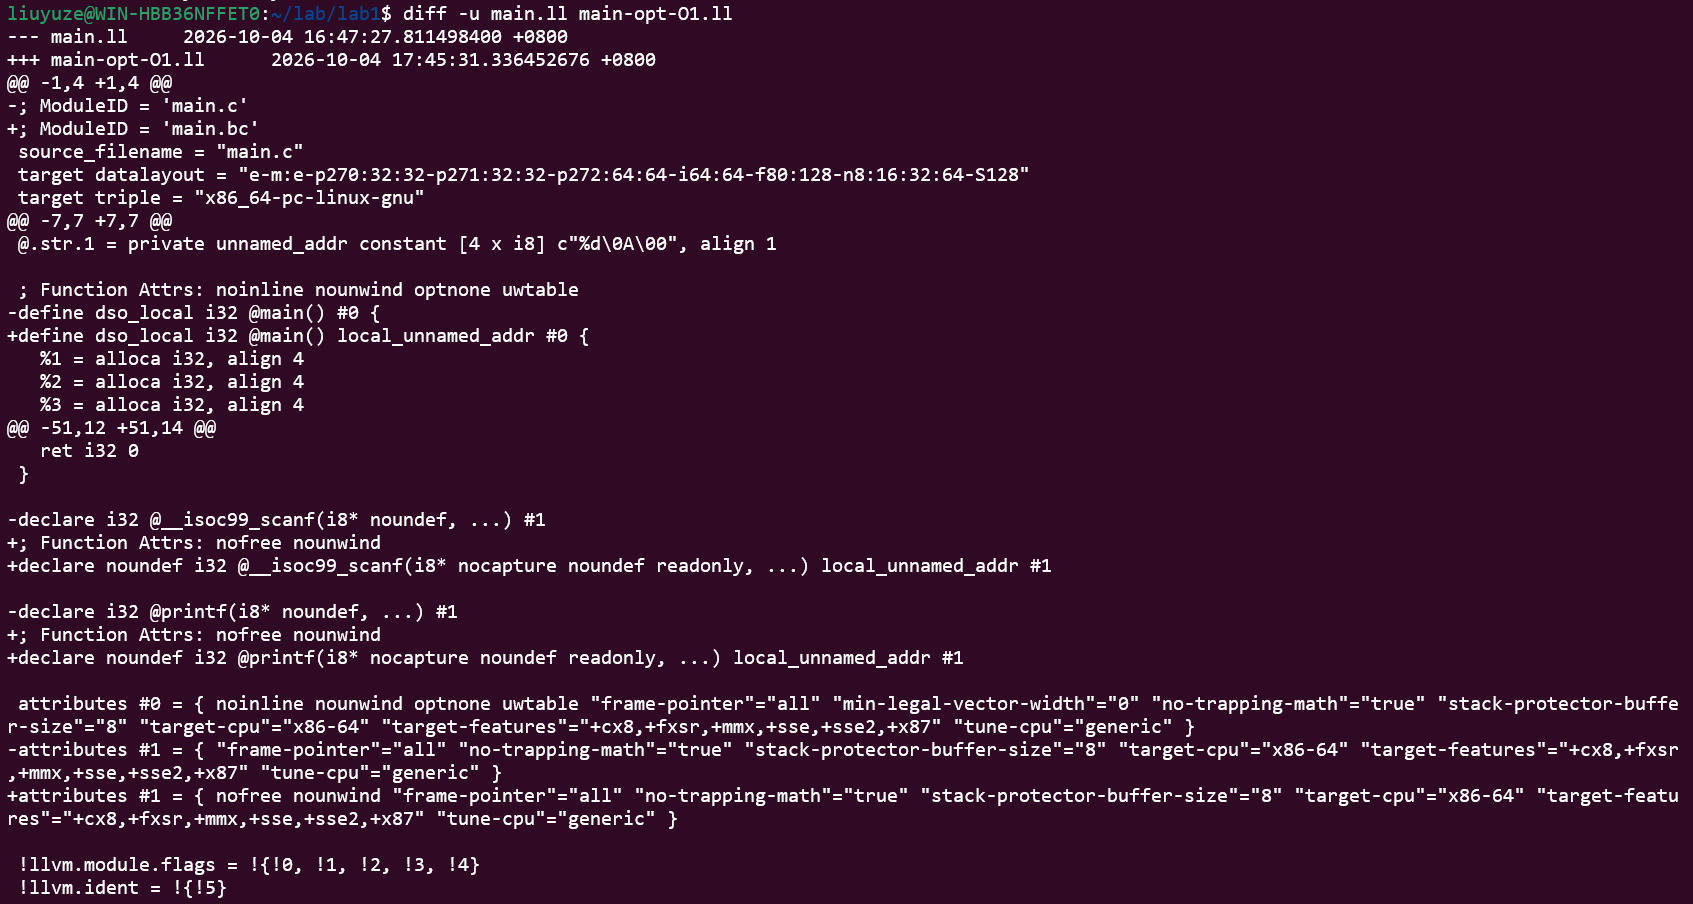
\includegraphics[width=\textwidth]{images/code-optimization-diff.png}
    \caption{优化前后的 LLVM IR 差异}
    \label{fig:code-optimization-diff}
\end{figure}

从差异可以看到，\verb|ModuleID| 由 \verb|main.c| 变为 \verb|main.bc|，这是
文本 IR 转换为位码后再次输出的结果。\verb|main| 的定义增加了
\verb|local_unnamed_addr| 属性，\verb|scanf| 和 \verb|printf| 的声明增加了
\verb|noundef|、\verb|nocapture|、\verb|readonly| 和
\verb|local_unnamed_addr| 等属性，属性组中同时增加了 \verb|nofree| 和
\verb|nounwind|。这些信息向优化器说明函数的地址是否重要、参数指向的内存是否
会被修改以及函数是否会抛出异常，从而为后续优化提供依据。

需要注意，此时 \verb|main| 仍然带有未优化编译产生的 \verb|optnone| 属性：

\begin{minted}{text}
; Function Attrs: noinline nounwind optnone uwtable
define dso_local i32 @main() local_unnamed_addr #0 {
\end{minted}

因此，\verb|opt| 不能深入优化 \verb|main| 的函数体，只能修改函数和库声明的
属性。差异中出现的主要变化是属性和地址标记，而不是 \verb|while| 循环被整体
替换。这个结果说明优化 pass 会受到函数属性的限制，也为下一步从源码开始使用
不同优化级别生成 IR 提供了对照。

\textbf{实验二：比较不同优化级别生成的 IR}

为了观察真正的循环优化效果，需要让 Clang 在生成 IR 时直接启用优化。依次执行：

\begin{minted}{bash}
clang -S -emit-llvm -O0 main.c -o main-O0.ll
clang -S -emit-llvm -O1 main.c -o main-O1.ll
clang -S -emit-llvm -O2 main.c -o main-O2.ll
clang -S -emit-llvm -O3 main.c -o main-O3.ll

wc -l main-O0.ll main-O1.ll main-O2.ll main-O3.ll
\end{minted}


分别查看未优化和 O1 优化后的 \verb|main| 函数：

\begin{minted}{bash}
sed -n '/^define dso_local i32 @main/,/^}/p' main-O0.ll
sed -n '/^define dso_local i32 @main/,/^}/p' main-O1.ll
\end{minted}

两张截图分别保存为 \verb|code-optimization-o0.png| 和
\verb|code-optimization-o1.png|。

\begin{figure}[H]
    \centering
    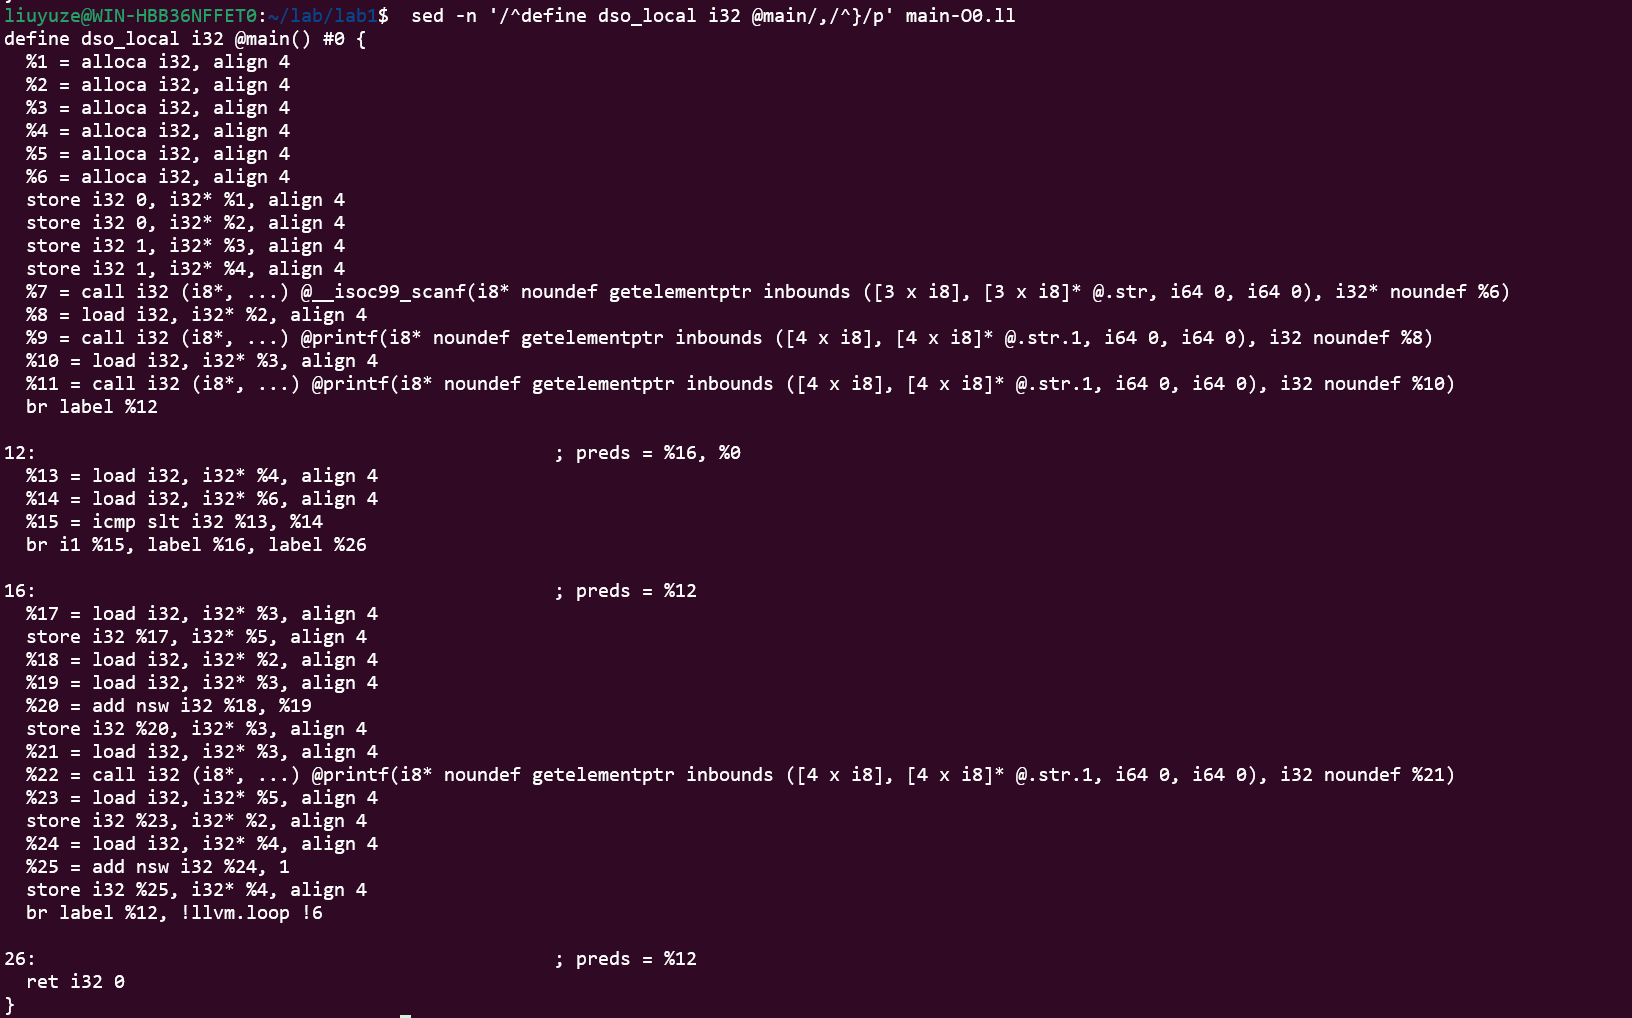
\includegraphics[width=\textwidth]{images/code-optimization-o0.png}
    \caption{\texttt{-O0} 生成的主函数 IR}
    \label{fig:code-optimization-o0}
\end{figure}

\begin{figure}[H]
    \centering
    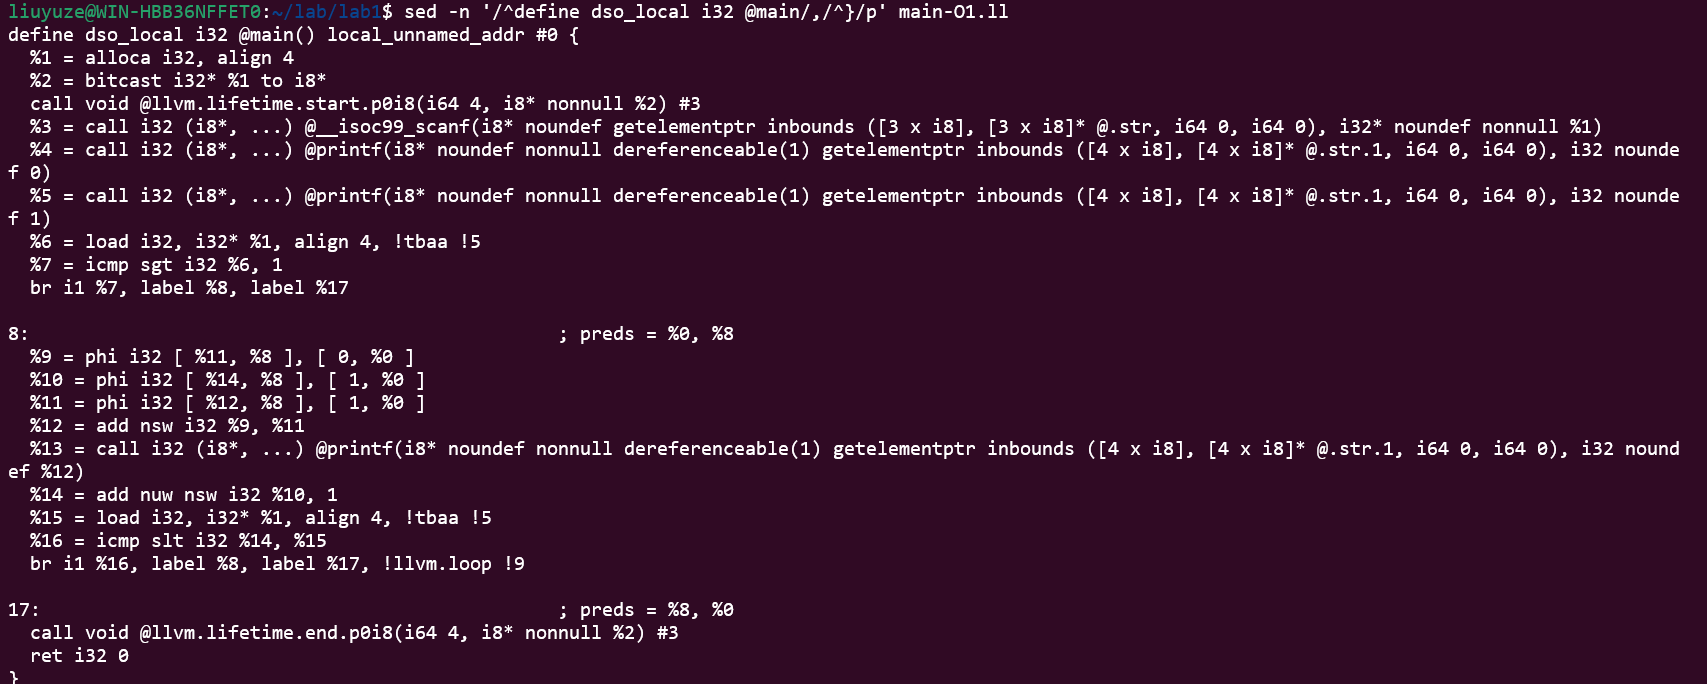
\includegraphics[width=\textwidth]{images/code-optimization-o1.png}
    \caption{\texttt{-O1} 优化后的主函数 IR}
    \label{fig:code-optimization-o1}
\end{figure}

未优化的 \verb|main-O0.ll| 为每个局部变量分配栈空间，反复使用
\verb|alloca|、\verb|load| 和 \verb|store| 完成变量读写，例如 \verb|a|、
\verb|b|、\verb|i| 和 \verb|t| 都通过栈位置保存。O1 优化后，这些变量的
栈存储基本被消除；变量 \verb|n| 仍需保留一个 \verb|alloca|，因为它要接收
\verb|scanf| 写入的地址。函数入口直接使用常量 \verb|0| 和 \verb|1| 完成前
两次输出，循环中的变量状态改用 \verb|phi| 指令保存。循环初值 \verb|i = 1|
和条件 \verb|i < n| 还被合并为入口处的 \verb|n > 1| 判断：

\begin{minted}{text}
%1 = alloca i32, align 4
%2 = bitcast i32* %1 to i8*
call void @llvm.lifetime.start.p0i8(i64 4, i8* nonnull %2) #3
%3 = call i32 (i8*, ...) @__isoc99_scanf(
        i8* noundef getelementptr inbounds ([3 x i8], [3 x i8]* @.str,
        i64 0, i64 0), i32* noundef nonnull %1)
%4 = call i32 (i8*, ...) @printf(
        i8* noundef nonnull dereferenceable(1)
        getelementptr inbounds ([4 x i8], [4 x i8]* @.str.1,
        i64 0, i64 0), i32 noundef 0)
%5 = call i32 (i8*, ...) @printf(
        i8* noundef nonnull dereferenceable(1)
        getelementptr inbounds ([4 x i8], [4 x i8]* @.str.1,
        i64 0, i64 0), i32 noundef 1)
%6 = load i32, i32* %1, align 4, !tbaa !5
%7 = icmp sgt i32 %6, 1
br i1 %7, label %8, label %17

8:
  %9  = phi i32 [ %11, %8 ], [ 0, %0 ]
  %10 = phi i32 [ %14, %8 ], [ 1, %0 ]
  %11 = phi i32 [ %12, %8 ], [ 1, %0 ]
  %12 = add nsw i32 %9, %11
  %13 = call i32 (i8*, ...) @printf(
        i8* noundef nonnull dereferenceable(1)
        getelementptr inbounds ([4 x i8], [4 x i8]* @.str.1,
        i64 0, i64 0),
        i32 noundef %12)
  %14 = add nuw nsw i32 %10, 1
  %15 = load i32, i32* %1, align 4, !tbaa !5
  %16 = icmp slt i32 %14, %15
  br i1 %16, label %8, label %17, !llvm.loop !9

17:
  call void @llvm.lifetime.end.p0i8(i64 4, i8* nonnull %2) #3
  ret i32 0
\end{minted}

其中，\verb|phi| 根据前驱基本块选择循环变量当前值；\verb|add nsw|
对应斐波那契数列加法；\verb|add nuw nsw| 对应
\verb|FIB_NEXT(i)| 展开后的自增操作；\verb|llvm.lifetime.start| 和
\verb|llvm.lifetime.end| 只用于标记局部存储对象的生命周期，不参与输入输出
计算。可以看到，O1 已经完成了大部分栈存储消除、常量替换和循环状态合并，
而不是只修改函数的属性。

\textbf{实验三：比较不同优化级别下的运行时间}

为了比较优化效果，新建 \verb|bench.c|:

\begin{minted}[frame=single, linenos=true]{c}
#include <stdio.h>
#include <stdint.h>
#include <time.h>

static volatile uint64_t sink;

int main(void)
{
    int n, trials;

    if (scanf("%d%d", &n, &trials) != 2 || n < 1 || trials < 1)
        return 1;

    clock_t start = clock();

    for (int k = 0; k < trials; ++k)
    {
        int a = 0, b = 1, i = 1, t;

        while (i < n)
        {
            t = b;
            b = a + b;
            a = t;
            i = i + 1;
        }

        sink += (uint64_t)(unsigned int)b;
    }

    clock_t end = clock();
    double total = (double)(end - start) / CLOCKS_PER_SEC;

    printf("n=%d trials=%d total=%.6f average=%.9f sink=%llu\n",
           n, trials, total, total / trials,
           (unsigned long long)sink);

    return 0;
}
\end{minted}

使用相同源文件分别生成四个不同优化级别的可执行文件：

\begin{minted}{bash}
clang -O0 bench.c -o bench-O0
clang -O1 bench.c -o bench-O1
clang -O2 bench.c -o bench-O2
clang -O3 bench.c -o bench-O3

ls -lh bench-O0 bench-O1 bench-O2 bench-O3
\end{minted}



使用相同的输入运行四个程序:
\begin{minted}{bash}
printf "40 1000000\n" | ./bench-O0
printf "40 1000000\n" | ./bench-O1
printf "40 1000000\n" | ./bench-O2
printf "40 1000000\n" | ./bench-O3
\end{minted}

四次运行的输出如图所示。每次输出的 \verb|sink| 均为
\verb|1023341550000000|，说明不同优化级别计算得到的斐波那契结果一致，
优化没有改变程序的运行结果。

\begin{figure}[H]
    \centering
    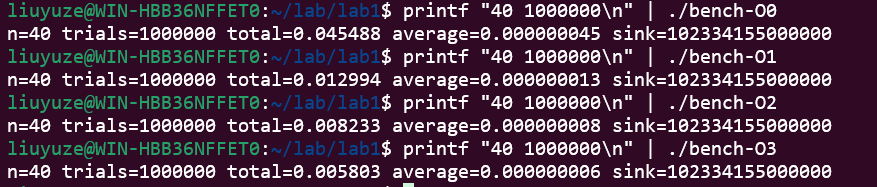
\includegraphics[width=\textwidth]{images/code-optimization-bench-result.png}
    \caption{不同优化级别的运行时间}
    \label{fig:code-optimization-bench-result}
\end{figure}



从结果可以看出，O1 的运行时间约为 O0 的 0.29 倍，加速约 3.50 倍；O2
约为 O0 的 0.18 倍，加速约 5.53 倍；O3 约为 O0 的 0.13 倍，加速约
7.84 倍。性能变化与前面的 IR 分析相互对应：O0 反复使用栈空间完成变量
读写，O1 开始使用寄存器状态的 \verb|phi| 合并、常量替换和循环简化，O2
与 O3 在此基础上继续精简和调度循环指令。


\textbf{(6)代码生成}

代码生成以中间表示形式为输入，将其映射为目标机器的汇编代码。使用
\verb|llc| 从 \verb|main.ll| 生成目标代码，再使用 \verb|clang -S| 生成
x86 汇编代码：

代码生成以中间表示形式为输入，将其映射为目标机器的汇编代码。本次实验使用
\verb|llc| 从 \verb|main.ll| 生成目标代码，再分别生成 x86 和 ARM 汇编代码：

\begin{minted}{bash}

llc main.ll -o main-llvm.S
gcc main.i -S -o main-x86.S
arm-linux-gnueabihf-gcc main.i -S -o main-arm.S
ls -lh main-llvm.S main-x86.S main-arm.S
\end{minted}

生成结果如图 \ref{fig:code-generation-files} 所示。

\begin{figure}[H]
    \centering
    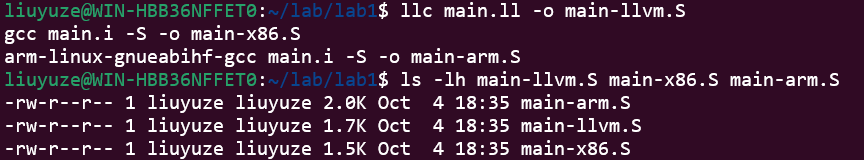
\includegraphics[width=0.75\textwidth]{images/code-generation-files.png}
    \caption{代码生成}
    \label{fig:code-generation-files}
\end{figure}




\subsubsection{汇编器}

汇编过程实际上把汇编语言程序代码翻译成目标机器指令的过程，其最终生成的是可重定位的机器代码。汇编器会将汇编程序中的伪指令翻译成等价的机器语言指令，将程序中的分支和数据传输指令中用到的标号都放到一个符号表中，我们通过查表可以生成对应指令的二进制。

我们使用汇编文件 \texttt{fib.s} 进行汇编，并通过 \texttt{objdump -d} 对 \texttt{fib.o} 进行反汇编，结果如图~\ref{fig:disasm} 所示。可以看到，\texttt{main} 函数的地址从 0 开始，说明尚未链接。

\begin{figure}[H]
    \centering
    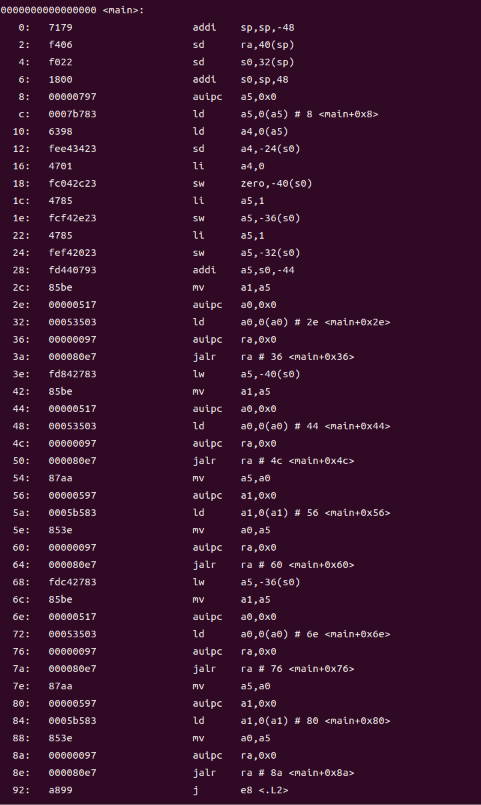
\includegraphics[width=0.6\textwidth]{images/figY.png}
    \caption{fib.o 反汇编结果}
    \label{fig:disasm}
\end{figure}

\texttt{nm} 命令显示的符号表如图~\ref{fig:symbol} 所示，\texttt{T main} 表示已定义的全局代码符号，\texttt{U} 开头的表示未定义、需要链接时解析的外部符号。

\begin{figure}[H]
    \centering
    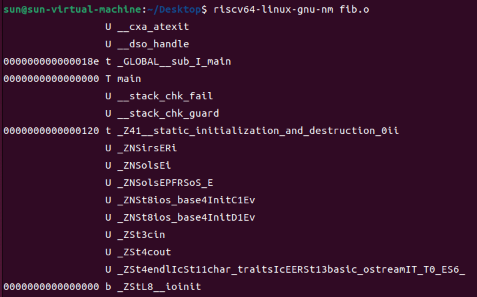
\includegraphics[width=0.8\textwidth]{images/figZ.png}
    \caption{fib.o 符号表}
    \label{fig:symbol}
\end{figure}

\texttt{objdump -r} 显示的重定位表如图~\ref{fig:reloc} 所示，记录了 \texttt{.text} 中需要在链接时修正的位置

\begin{figure}[H]
    \centering
    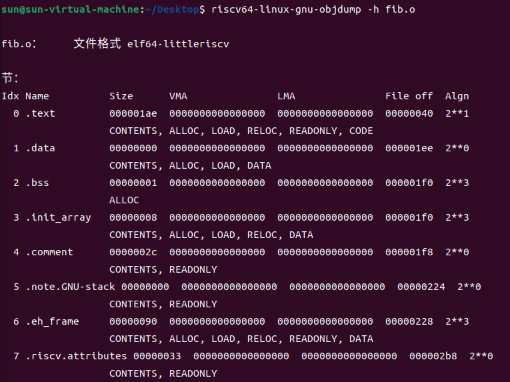
\includegraphics[width=0.8\textwidth]{images/figW.png}
    \caption{fib.o 重定位表}
    \label{fig:reloc}
\end{figure}

综上，汇编器完成了从汇编到可重定位目标文件的翻译，并留下符号表和重定位信息，供链接器使用。


\subsubsection{链接器}

由汇编程序生成的目标文件不能够直接执行。大型程序常常被分成多个部分进行编译，因此，可重定位的机器代码有必要和其他可重定位的目标文件以及库文件链接到一起，最终形成真正在机器上运行的代码。进而链接器对该机器代码进行执行生成可执行文件。

我们使用如下命令将 \texttt{fib.o} 链接为可执行文件 \texttt{fib}：

\begin{lstlisting}[language=bash]
riscv64-linux-gnu-g++ fib.o -o fib -static
\end{lstlisting}

使用 \texttt{file} 命令查看生成的可执行文件，如图~\ref{fig:file} 所示，可以看到它是一个 RISC-V 架构的 ELF 可执行文件。

\begin{figure}[H]
    \centering
    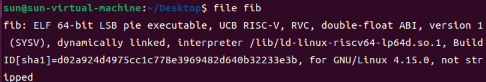
\includegraphics[width=0.6\textwidth]{images/fig_link_file.png}
    \caption{file 命令查看可执行文件}
    \label{fig:file}
\end{figure}

我们使用 \texttt{objdump -d} 对 \texttt{fib} 进行反汇编，得到 \texttt{main} 函数的反汇编结果，如图~\ref{fig:link_disasm} 所示。可以看到，与汇编器阶段生成的目标文件不同，此时 \texttt{main} 函数的地址不再是 0，而是链接后分配的实际虚拟地址；\texttt{call} 指令的目标地址也已经被链接器填上。

\begin{figure}[H]
    \centering
    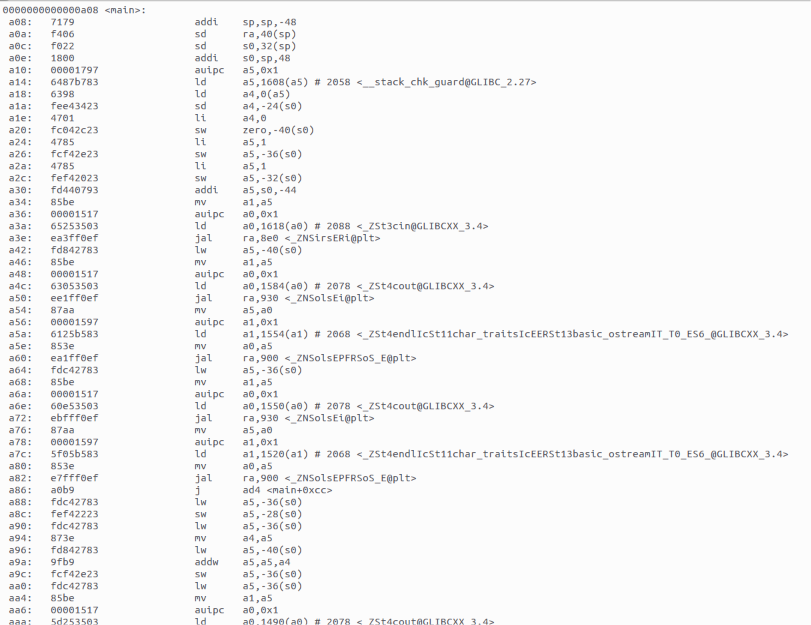
\includegraphics[width=0.8\textwidth]{images/fig_link_disasm.png}
    \caption{链接后 main 函数反汇编}
    \label{fig:link_disasm}
\end{figure}

使用 \texttt{nm} 查看符号表，如图~\ref{fig:link_nm} 所示，原来在目标文件中标记为 \texttt{U} 的未定义符号，在链接后已经被解析，或者标记为从动态库导入。

\begin{figure}[H]
    \centering
    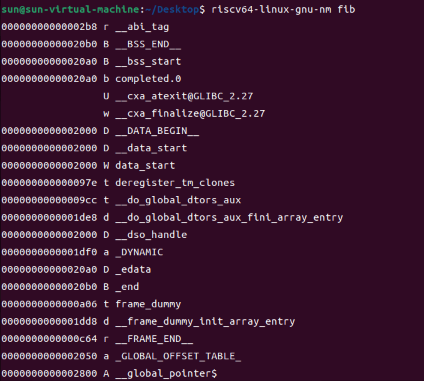
\includegraphics[width=0.8\textwidth]{images/fig_link_nm.png}
    \caption{链接后符号表}
    \label{fig:link_nm}
\end{figure}

使用 \texttt{objdump -h} 查看段表，如图~\ref{fig:link_sections} 所示。

\begin{figure}[H]
    \centering
    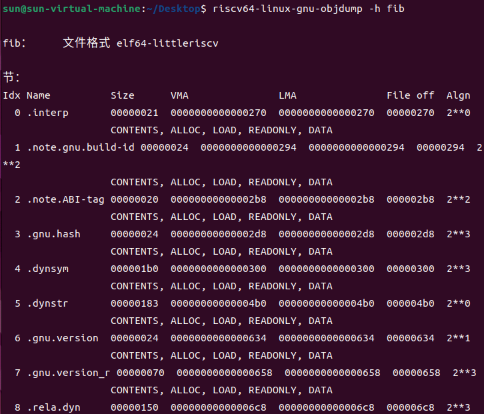
\includegraphics[width=0.8\textwidth]{images/fig_link_sections.png}
    \caption{链接后段表}
    \label{fig:link_sections}
\end{figure}

进一步查看 \texttt{.plt} 节的反汇编，如图~\ref{fig:link_plt} 所示。\texttt{.plt}（Procedure Linkage Table）是用于动态链接的跳转指令表，包含了从程序代码到动态库中函数实现的间接跳转。链接器在链接时补上了之前的空白地址，实现了将目标文件和库文件链接到一起的功能。

\begin{figure}[H]
    \centering
    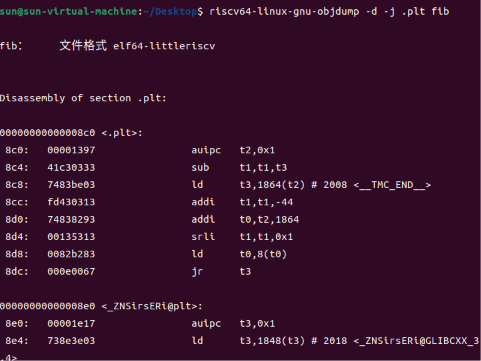
\includegraphics[width=0.8\textwidth]{images/fig_link_plt.png}
    \caption{.plt 节反汇编}
    \label{fig:link_plt}
\end{figure}

综上，链接器完成了符号解析和地址重定位，将多个目标文件和库文件合并成一个可执行文件，为程序的最终运行做好了准备。

%——————————————————————————————————————
\subsection{熟悉LLVM IR中间语言}

LLVM IR是LLVM编译器框架的中间表示形式，具有类型化、可扩展、强表现力等特点。它有三种表示形式：内存中的对象、二进制bitcode（.bc）和可读的文本形式（.ll）。本实验通过编写一个简单的LLVM IR程序，并链接SysY运行时库，来熟悉LLVM IR的基本语法与程序结构。

\subsubsection{实验程序}

我们编写了一个计算阶乘的LLVM IR程序\texttt{main.ll}，它调用SysY运行时库提供的\texttt{getint}、\texttt{putint}、\texttt{putch}函数完成输入输出。程序源码如图~\ref{fig:llvm_ir_code}所示。

\begin{figure}[H]
    \centering
    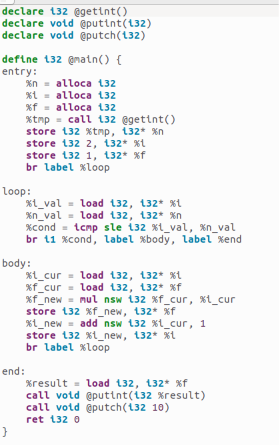
\includegraphics[width=0.4\textwidth]{images/fig_llvm_ir_code.png}
    \caption{LLVM IR阶乘程序main.ll}
    \label{fig:llvm_ir_code}
\end{figure}

\subsubsection{编译与链接}

使用\texttt{clang}将LLVM IR文件编译为目标文件，再用RISC-V工具链链接SysY运行时库，生成可执行文件。命令如下：

\begin{lstlisting}[language=bash]
clang --target=riscv64-unknown-linux-gnu -c main.ll -o main.o
riscv64-unknown-elf-gcc main.o ~/lib/libsysy_riscv.a -o main -static
\end{lstlisting}

生成的可执行文件\texttt{main}为RISC-V架构，如图~\ref{fig:llvm_link} 所示。

\begin{figure}[H]
    \centering
    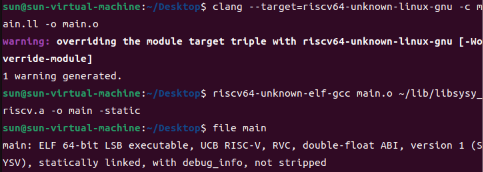
\includegraphics[width=0.7\textwidth]{images/fig_llvm_link.png}
    \caption{编译链接命令及file命令查看可执行文件}
    \label{fig:llvm_link}
\end{figure}

\subsubsection{运行验证}

使用QEMU运行程序，输入\texttt{5}，程序输出\texttt{120}，结果正确，如图~\ref{fig:llvm_run}所示。

\begin{figure}[H]
    \centering
    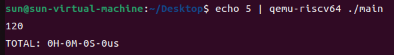
\includegraphics[width=0.6\textwidth]{images/fig_llvm_run.png}
    \caption{LLVM IR程序运行结果}
    \label{fig:llvm_run}
\end{figure}

通过本实验，我们了解了LLVM IR的基本结构，包括函数定义、基本块、虚拟寄存器、类型系统、分支与指令等，并掌握了将LLVM IR与SysY运行时库链接并执行的方法。
%——————————————————————————————————————
\subsection{熟悉汇编语言}

以斐波那契数列程序为例，使用 RISC-V 汇编语言实现与 C 程序相同的功能。
源程序 \verb|fibonacci.c| 如下：

\subsubsection{实验程序}

\begin{minted}[frame=single, linenos=true]{c}
#include <stdio.h>

int main()
{
    int a, b, i, t, n;

    a = 0;
    b = 1;
    i = 1;

    scanf("%d", &n);

    printf("%d\n", a);
    printf("%d\n", b);

    while (i < n)
    {
        t = b;
        b = a + b;
        printf("%d\n", b);
        a = t;
        i = i + 1;
    }

    return 0;
}
\end{minted}

\textbf{RISC-V 汇编实现}


主要寄存器分配如下：

\begin{center}
\begin{tabular}{cl}
    \toprule
    寄存器 & 保存内容 \\
    \midrule
    \verb|s0| & 变量 \verb|a| \\
    \verb|s1| & 变量 \verb|b| \\
    \verb|s2| & 变量 \verb|i| \\
    \verb|s3| & 临时变量 \verb|t| \\
    \verb|s4| & 输入变量 \verb|n| \\
    \verb|a0|、\verb|a1| & 函数参数 \\
    \verb|ra| & 返回地址 \\
    \bottomrule
\end{tabular}
\end{center}

完整的 RISC-V 汇编程序 \verb|fibonacci.s| 如下：

\begin{minted}[frame=single, linenos=true, breaklines, breakanywhere]{asm}
    .option nopic
    .attribute arch, "rv64gc"
    .attribute unaligned_access, 0
    .attribute stack_align, 16

    .section .rodata
    .align 3
.LC0:
    .string "%d"
    .align 3
.LC1:
    .string "%d\n"

    .text
    .align 1
    .globl main
    .type main, @function

main:
    addi sp, sp, -64
    sd ra, 56(sp)
    sd s0, 48(sp)
    sd s1, 40(sp)
    sd s2, 32(sp)
    sd s3, 24(sp)
    sd s4, 16(sp)

    # a = 0, b = 1, i = 1
    li s0, 0
    li s1, 1
    li s2, 1

    # scanf("%d", &n)
    lui a0, %hi(.LC0)
    addi a0, a0, %lo(.LC0)
    addi a1, sp, 8
    call scanf
    lw s4, 8(sp)

    # 输出初始值 a
    lui a0, %hi(.LC1)
    addi a0, a0, %lo(.LC1)
    mv a1, s0
    call printf

    # 输出初始值 b
    lui a0, %hi(.LC1)
    addi a0, a0, %lo(.LC1)
    mv a1, s1
    call printf

.Lloop:
    # if (i >= n) 结束循环
    bge s2, s4, .Lend

    # t = b; b = a + b
    mv s3, s1
    add s1, s0, s1

    # printf("%d\n", b)
    lui a0, %hi(.LC1)
    addi a0, a0, %lo(.LC1)
    mv a1, s1
    call printf

    # a = t; i = i + 1
    mv s0, s3
    addi s2, s2, 1
    j .Lloop

.Lend:
    # return 0
    li a0, 0

    ld ra, 56(sp)
    ld s0, 48(sp)
    ld s1, 40(sp)
    ld s2, 32(sp)
    ld s3, 24(sp)
    ld s4, 16(sp)
    addi sp, sp, 64
    ret

    .size main, .-main
    .section .note.GNU-stack,"",@progbits
\end{minted}

程序进入 \verb|main| 后，首先将 \verb|ra| 和 \verb|s0| 到 \verb|s4| 保存到
栈中，再完成变量初始化。调用 \verb|scanf| 时，\verb|a0| 保存格式字符串
\verb|"%d"| 的地址，\verb|a1| 保存变量 \verb|n| 在栈中的地址；输入完成后，
\verb|lw s4, 8(sp)| 将 \verb|n| 的值读入寄存器 \verb|s4|。两次
\verb|printf| 的调用方式相同，\verb|a0| 传入格式字符串，\verb|a1| 传入待输出
的整数值。

循环开始处的 \verb|bge s2, s4, .Lend| 表示当 \verb|i >= n| 时退出循环，因此
等价于 C 语言中的 \verb|while (i < n)|。循环体中，\verb|mv s3, s1| 保存旧的
\verb|b|，\verb|add s1, s0, s1| 完成 \verb|b = a + b|；输出新的 \verb|b|
后，\verb|mv s0, s3| 和 \verb|addi s2, s2, 1| 分别完成 \verb|a = t| 和
\verb|i = i + 1|。最后使用 \verb|j .Lloop| 跳回循环条件处。

程序结束时，将 \verb|a0| 置为 0 作为返回值，依次恢复保存过的寄存器，使用
\verb|addi sp, sp, 64| 释放栈空间，最后通过 \verb|ret| 返回调用者。

\subsubsection{运行验证}

使用 RISC-V 交叉编译器和 QEMU 运行程序：

\begin{minted}{bash}
fibonacci.s -o fibonacci -static
qemu-riscv64 fibonacci
\end{minted}

输入 \verb|12| 后，终端依次输出从 0 开始的斐波那契数列，结果如图
\ref{fig:task3-fibonacci-run} 所示。

\begin{figure}[H]
    \centering
    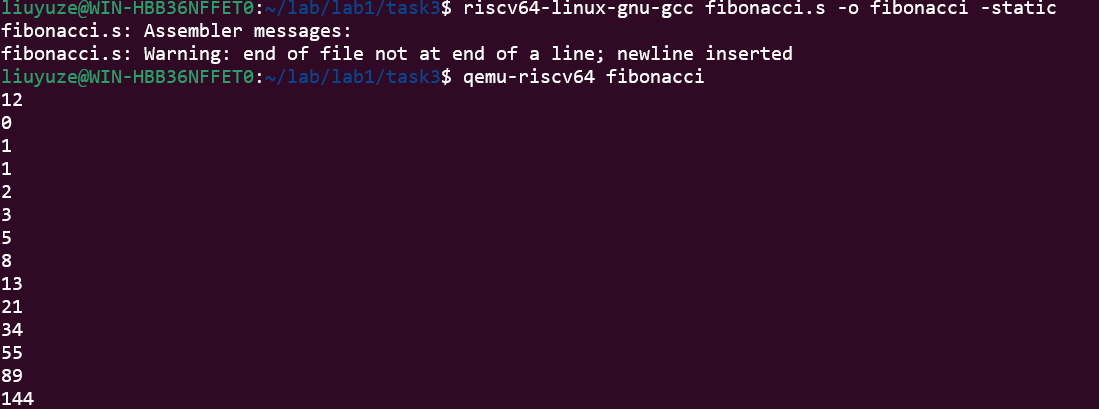
\includegraphics[width=0.8\linewidth]{images/task3-fibonacci-run.png}
    \caption{斐波那契汇编程序的运行结果}
    \label{fig:task3-fibonacci-run}
\end{figure}

汇编程序中的变量初始化、输入、循环计算和输出均正确。


\subsubsection{反汇编验证}

为了观察汇编器最终生成的目标指令，执行：

\begin{minted}{bash}
riscv64-linux-gnu-objdump -d fibonacci \
    | sed -n '/<main>:/,/^$/p'
\end{minted}

反汇编结果如图 \ref{fig:task3-fibonacci-objdump} 所示。

\begin{figure}[H]
    \centering
    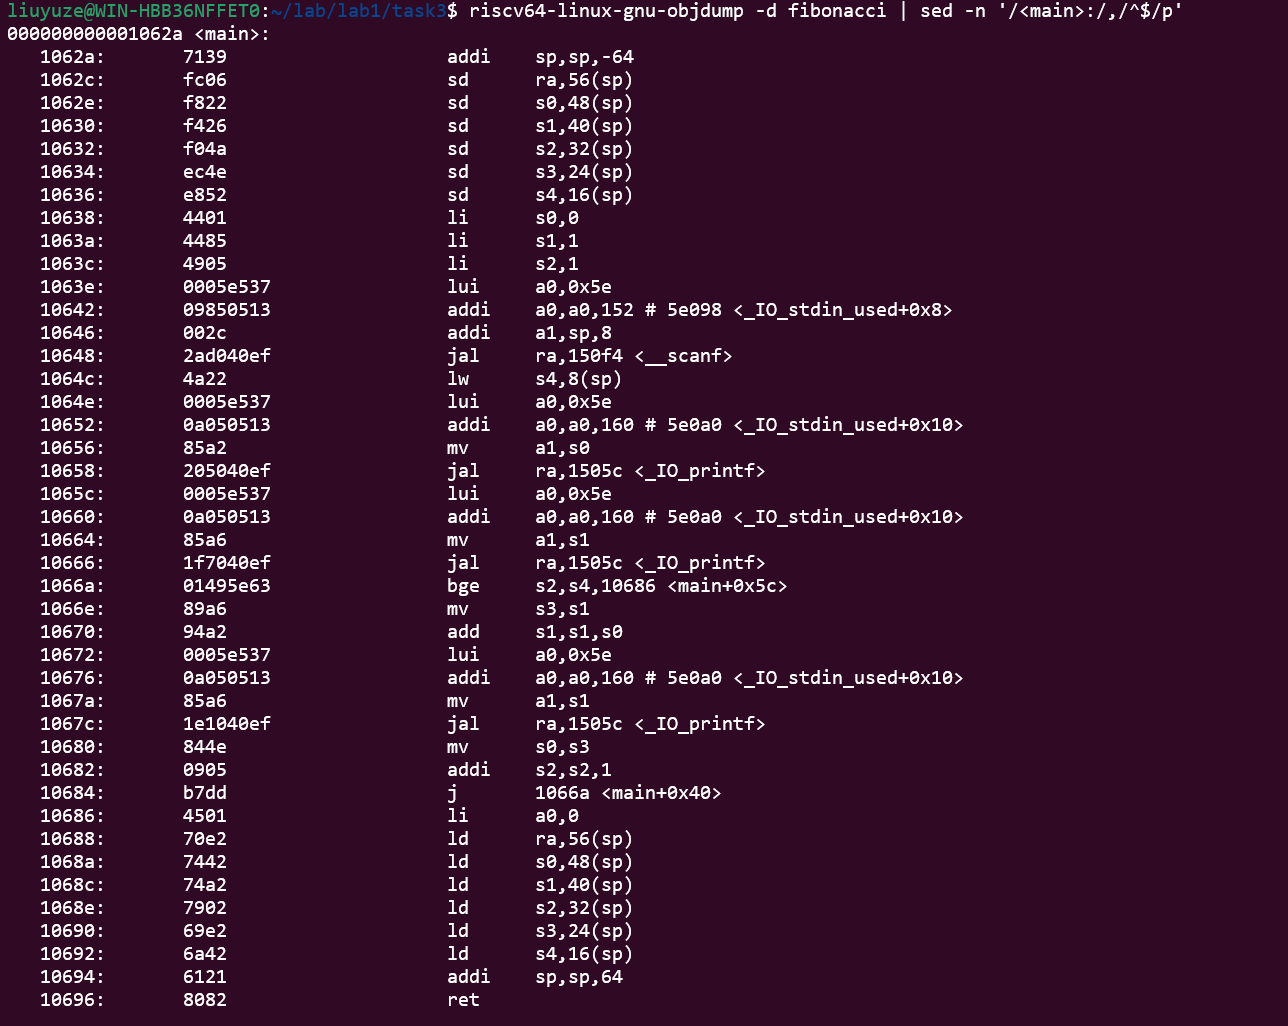
\includegraphics[width=\linewidth]{images/task3-fibonacci-objdump.png}
    \caption{斐波那契程序的反汇编结果}
    \label{fig:task3-fibonacci-objdump}
\end{figure}

反汇编结果与编写的汇编程序一致：\verb|li| 指令完成变量初值设置，
\verb|jal| 调用 \verb|scanf| 和 \verb|printf|，\verb|bge| 判断循环是否结束，
\verb|add|、\verb|addi|、\verb|mv| 完成斐波那契数列的计算和变量更新。
由于程序采用静态链接，反汇编中的 \verb|scanf| 和 \verb|printf| 分别显示为
\verb|__scanf| 和 \verb|_IO_printf|，但其调用功能不变。返回前，\verb|ld|
指令恢复保存的寄存器，\verb|addi sp, sp, 64| 释放栈帧，最后通过 \verb|ret|
返回。



%----------------------------------------------------------------
\newpage
\section{进阶要求}
%——————————————————————————————————————
\subsection{实验目的}

本部分以逐元素向量加法为例，观察 MLIR 如何把同一段程序从高层结构化表示
逐步降低为低层控制流和 LLVM 方言，并最终翻译成 LLVM IR。

\subsection{实验过程}

实验在 WSL Ubuntu 22.04 中进行，使用 \verb|mlir-opt-14| 和
\verb|mlir-translate-14|。测试用例 \verb|vecadd.mlir| 完成
\verb|C[i] = A[i] + B[i]| 的计算，三个数组均为
\verb|memref<16xi16>|。最开始的样例代码如下：

\begin{minted}{text}
#map = affine_map<(d0) -> (d0)>
module {
  func @vecadd(%arg0: memref<16xi16>, %arg1: memref<16xi16>,
               %arg2: memref<16xi16>) {
    linalg.generic {indexing_maps = [#map, #map, #map],
                    iterator_types = ["parallel"]}
        ins(%arg0, %arg1 : memref<16xi16>, memref<16xi16>)
        outs(%arg2 : memref<16xi16>) {
    ^bb0(%arg3: i16, %arg4: i16, %arg5: i16):
      %0 = arith.addi %arg3, %arg4 : i16
      linalg.yield %0 : i16
    }
    return
  }
}
\end{minted}

该样例用 \verb|linalg.generic| 描述逐元素加法。进入实验目录后，依次执行不同 lowering pass，
并保存每一阶段的输出：

\begin{minted}{bash}

mlir-opt-14 vecadd.mlir \
    | tee vecadd-high-level.mlir

mlir-opt-14 --convert-linalg-to-loops vecadd.mlir \
    | tee vecadd-linalg-to-loops.mlir

mlir-opt-14 --convert-linalg-to-loops --convert-scf-to-std \
    vecadd.mlir | tee vecadd-scf-to-cfg.mlir

mlir-opt-14 --convert-linalg-to-loops --convert-scf-to-std \
    --convert-std-to-llvm --convert-memref-to-llvm \
    --reconcile-unrealized-casts vecadd.mlir \
    | tee vecadd-llvm-dialect.mlir

mlir-translate-14 --mlir-to-llvmir \
    vecadd-llvm-dialect.mlir -o vecadd.ll
sed -n '1,120p' vecadd.ll
\end{minted}

\textbf{逐级降低过程}

最初的高层 MLIR 使用 \verb|linalg.generic| 描述向量加法。索引映射
\verb|affine_map<(d0) -> (d0)>| 表示输入和输出按同一维下标访问，
\verb|iterator_types = ["parallel"]| 表明该操作可以并行执行；计算体中的
\verb|arith.addi| 完成两个 \verb|i16| 元素相加。该层主要描述“做什么”，
尚未显式展开循环和内存访问。

\begin{figure}[H]
    \centering
    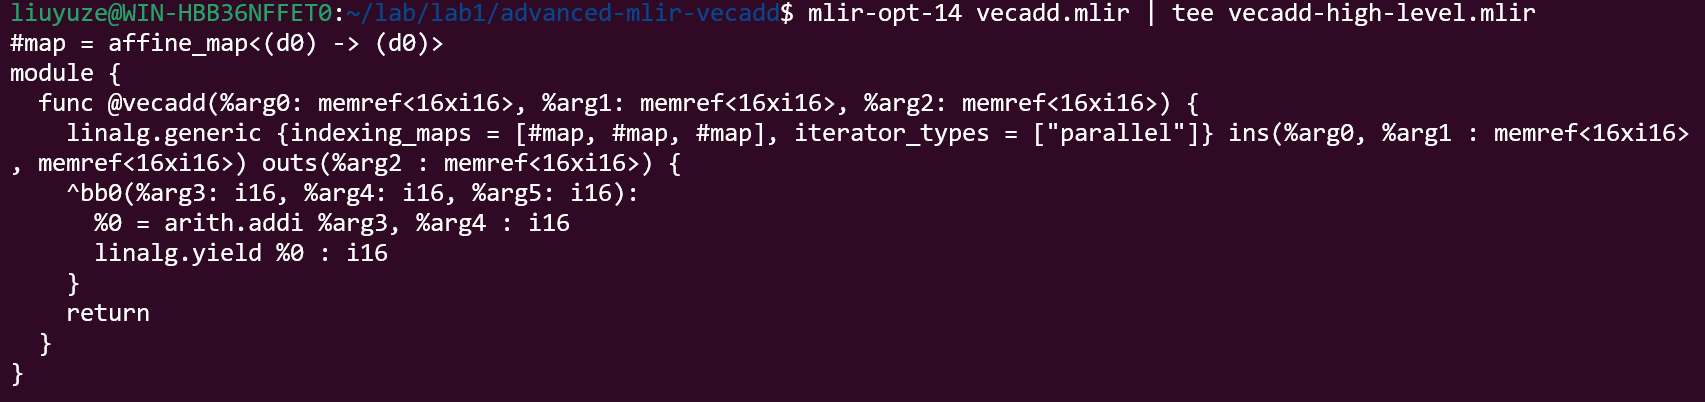
\includegraphics[width=\linewidth]{images/mlir-vecadd-high-level.png}
    \caption{VecAdd 的高层 Linalg MLIR}
    \label{fig:mlir-vecadd-high-level}
\end{figure}

执行 \verb|--convert-linalg-to-loops| 后，\verb|linalg.generic| 被转换为
\verb|scf.for| 循环。循环下界、上界和步长分别由 \verb|arith.constant|
给出，数组访问被展开为 \verb|memref.load| 和 \verb|memref.store|，
加法运算仍由 \verb|arith.addi| 完成。这一阶段把高层张量语义落实为显式
循环和标量访存，但控制流仍保持结构化形式。

\begin{figure}[H]
    \centering
    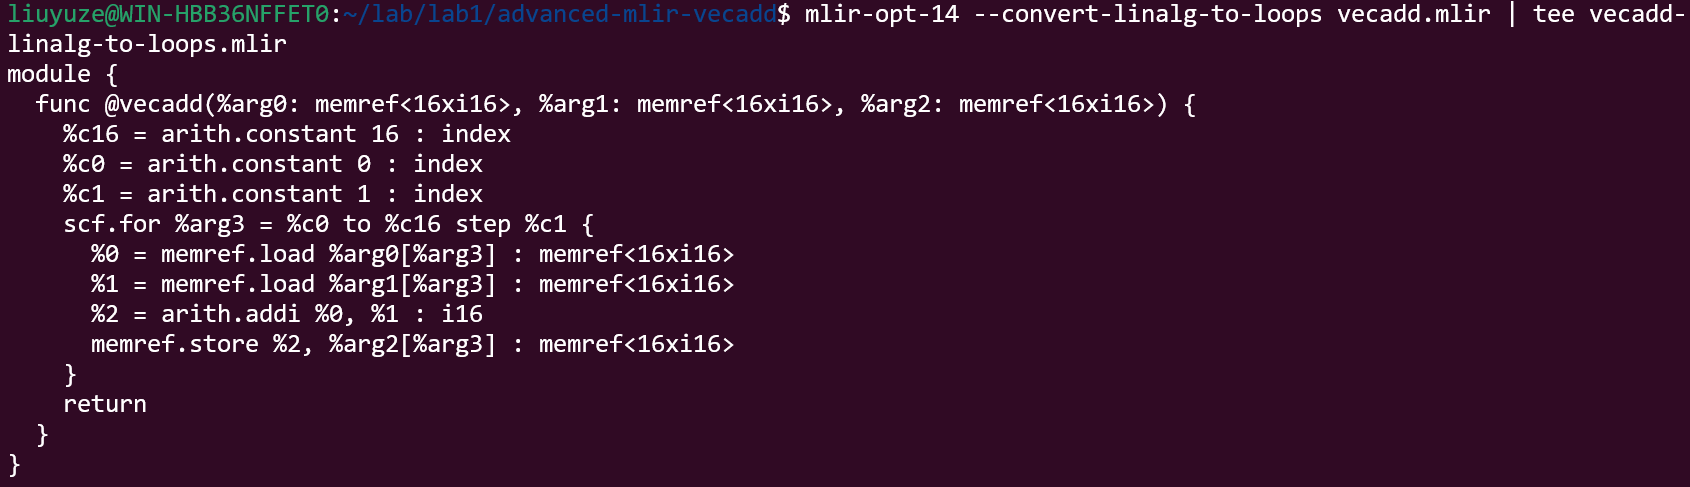
\includegraphics[width=\linewidth]{images/mlir-vecadd-linalg-to-loops.png}
    \caption{Linalg 降低为 SCF 循环后的 MLIR}
    \label{fig:mlir-vecadd-linalg-to-loops}
\end{figure}

继续执行 \verb|--convert-scf-to-std|，\verb|scf.for| 被展开为基本块和
分支指令。进入循环前使用 \verb|br| 跳转到条件判断块，循环条件由
\verb|arith.cmpi| 计算，随后通过 \verb|cond_br| 分别跳转到循环体和退出块。
循环体末尾再通过 \verb|br| 返回判断块，形成显式的 CFG。

\begin{figure}[H]
    \centering
    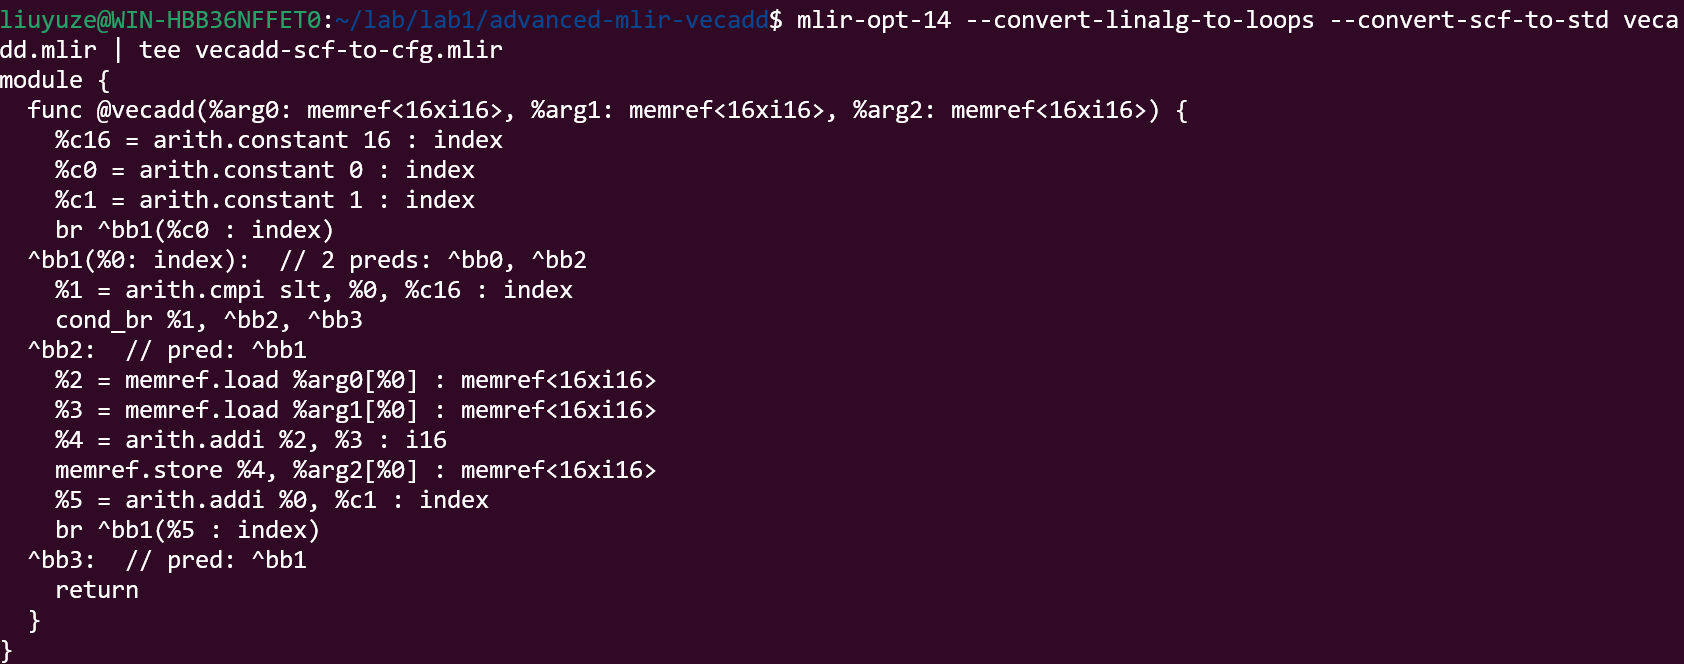
\includegraphics[width=\linewidth]{images/mlir-vecadd-scf-to-cfg.png}
    \caption{SCF 降低为 CFG 后的 MLIR}
    \label{fig:mlir-vecadd-scf-to-cfg}
\end{figure}

再经过 \verb|--convert-std-to-llvm|、\verb|--convert-memref-to-llvm| 和
\verb|--reconcile-unrealized-casts|，程序进一步降低到 LLVM 方言。
原来的函数、访存、算术和分支分别变为 \verb|llvm.func|、
\verb|llvm.getelementptr|、\verb|llvm.load|、\verb|llvm.add|、
\verb|llvm.store|、\verb|llvm.br| 和 \verb|llvm.cond_br|。此时程序已经
接近机器级表示，但仍保留在 MLIR 框架中。

\begin{figure}[H]
    \centering
    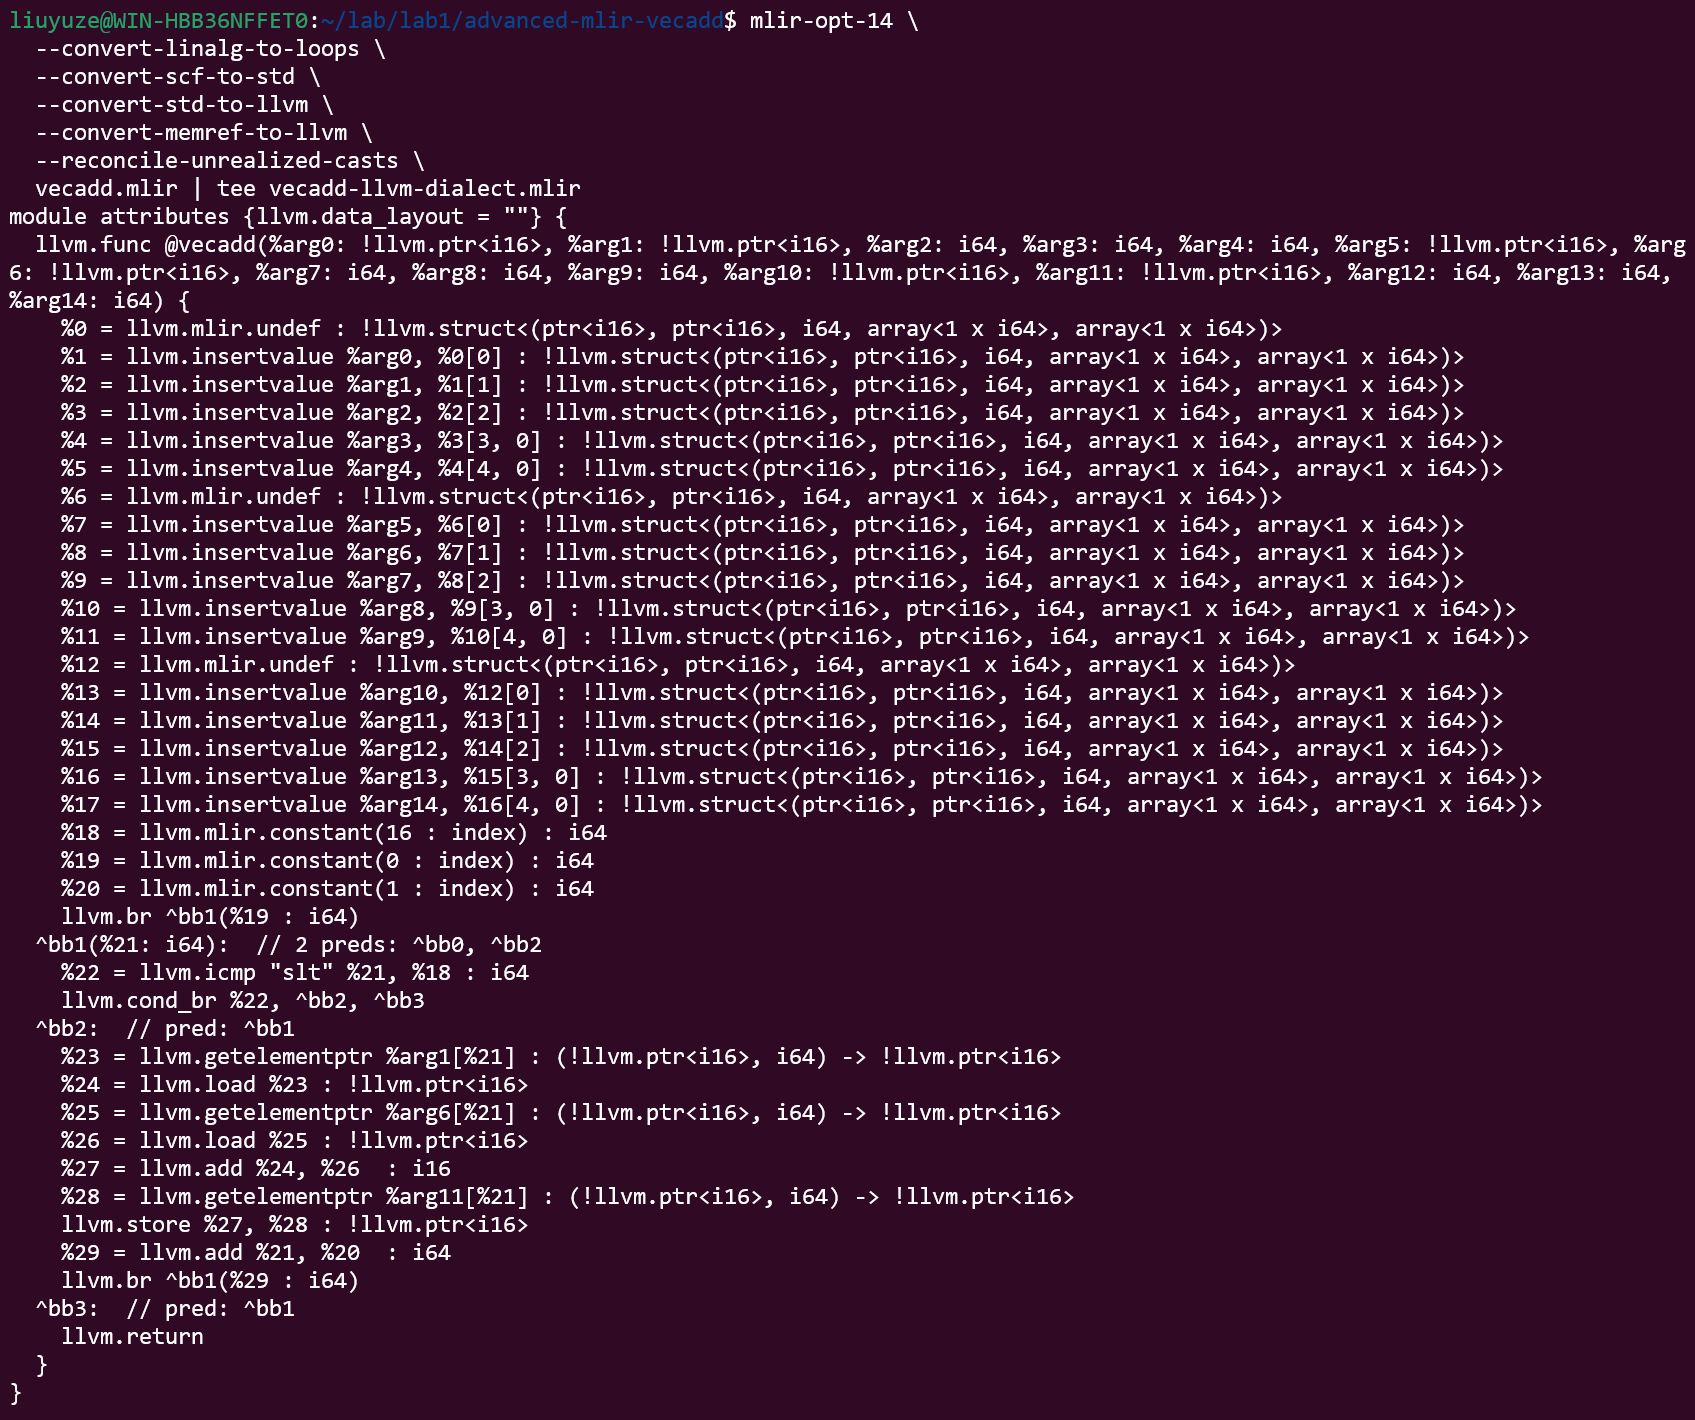
\includegraphics[width=\linewidth]{images/mlir-vecadd-llvm-dialect.png}
    \caption{VecAdd 降低为 LLVM 方言}
    \label{fig:mlir-vecadd-llvm-dialect}
\end{figure}

最后使用 \verb|mlir-translate-14 --mlir-to-llvmir| 将 LLVM 方言翻译为
标准 LLVM IR。输出中出现 \verb|define|、\verb|load|、\verb|add|、
\verb|store|、\verb|br| 和 \verb|ret| 等 LLVM IR 指令；循环变量在基本块
入口处通过 \verb|phi| 合并。至此，MLIR 完成了从高层方言到通用 LLVM IR
的转换，后续可以交给 LLVM 后端继续优化并生成目标机器代码。

\begin{figure}[H]
    \centering
    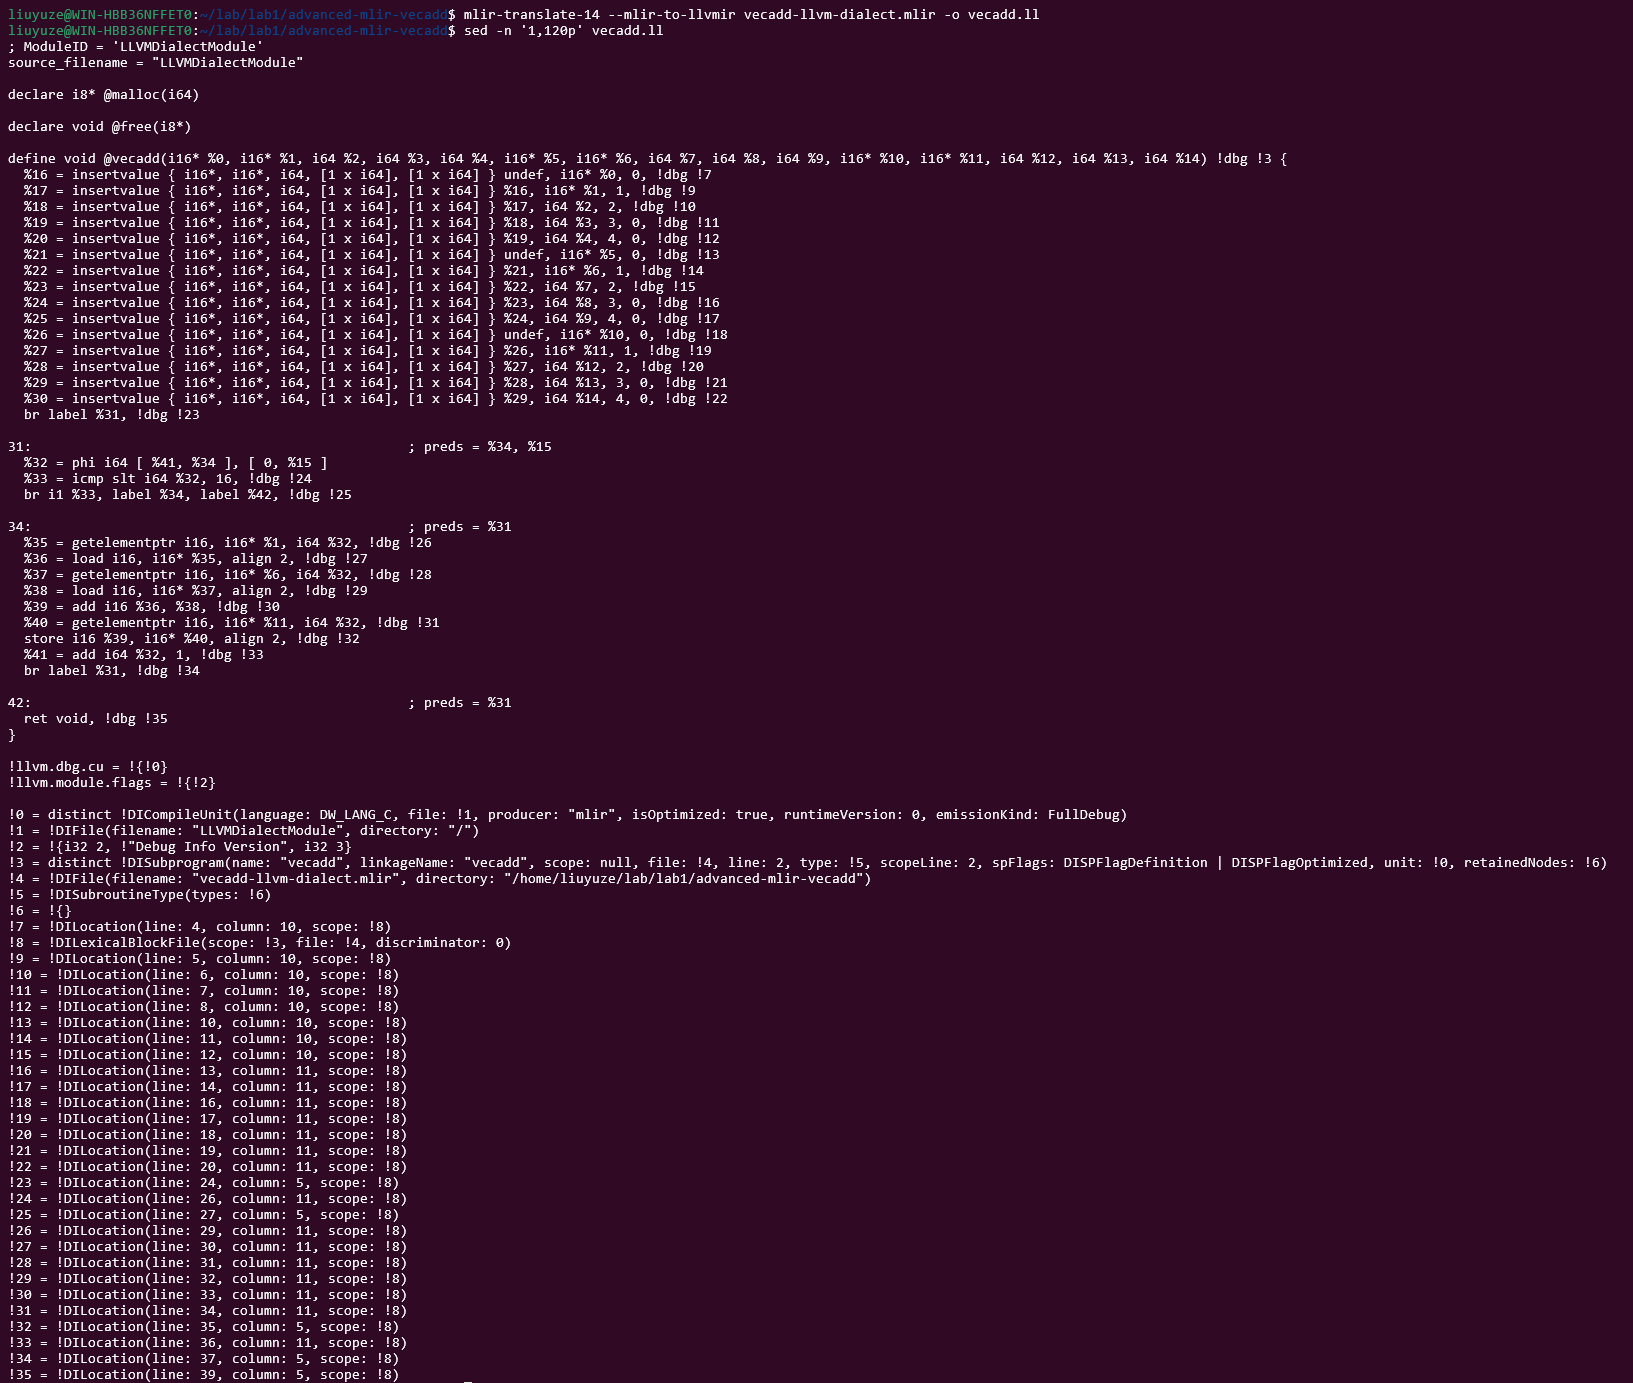
\includegraphics[width=\linewidth]{images/mlir-vecadd-llvm-ir.png}
    \caption{由 MLIR 翻译得到的 LLVM IR}
    \label{fig:mlir-vecadd-llvm-ir}
\end{figure}




\textbf{实验小结}

实验表明，MLIR 可以通过不同 dialect 和 pass 对同一语义进行渐进式降低：
\verb|linalg| 保留高层向量语义，\verb|scf| 显式描述结构化循环，
CFG 表示低层控制流，LLVM 方言则与通用后端衔接。AscendNPU IR 在通用
多级降低思想的基础上增加了面向 NPU 的算子和地址空间，使编译器能够在
保持中间表示可分析性的同时完成特定硬件后端映射。



%----------------------------------------------------------------
\newpage
\section{总结}

本次实验从完整编译流程出发，借助 GCC/Clang、LLVM 和 RISC-V 工具链分别完成了预处理、
编译、汇编和链接的观察与验证。在编译器内部，我们结合词法分析、语法分析、语义分析、
LLVM IR 生成以及不同优化级别的结果，理解了源代码到中间表示的转换；在目标代码阶段，
则通过汇编、反汇编、符号表和重定位信息，梳理了目标文件与可执行文件之间的联系。
最终，LLVM IR 阶乘程序和 RISC-V 斐波那契程序均运行正确，使我们对编译系统各阶段的
分工与协作有了更直观、完整的认识。

在进阶要求中，又通过 MLIR 观察了 VecAdd 从 Linalg、SCF、CFG 到 LLVM 方言和
LLVM IR 的逐级降低过程，并结合 AscendNPU IR 的示例理解了专用方言、硬件地址空间
和编译后端映射之间的关系，进一步认识到多级中间表示和 pass 机制在编译器中的衔接作用。

\noindent\textbf{仓库链接：}\url{https://github.com/liuyuze-121/nku-compiler-labs.git}

%----------------------------------------------------------------

\end{document}
